% v0.4 - 2011071901
%
% Modelo de monografia em LaTeX da UECE baseado no template disponibilizado
% por Rudy Matela em http://www.larces.uece.br/~rudy/pub/modelo_monografia/

\documentclass[pnumabnt,normaltoc,capchap,floatnumber=continuous]{abnt}		
\usepackage[bibjustif,abnt-etal-cite=3,abnt-etal-list=0,abnt-full-initials=yes]{abntcite}
\usepackage{modelo/tex/uece}
\usepackage[portuguese,brazilian,portuges]{babel}
\usepackage[utf8]{inputenc}
\usepackage{abnt-alf}
\usepackage{graphicx}
\usepackage{multicol}
\usepackage{listings}
\usepackage{booktabs}
\usepackage{amsmath}
\usepackage{amsthm}
\usepackage{eucal}
\usepackage{amssymb}
\usepackage{mathrsfs}
\usepackage[notintoc,portuguese]{nomencl}
\usepackage[section]{placeins}
\usepackage{algpseudocode,algorithm}
\bibliographystyle{abnt-alf}

\usepackage{xcolor}
\definecolor{verde}{rgb}{0.25,0.5,0.35}
\definecolor{jpurple}{rgb}{0.5,0,0.35}
\definecolor{dkgreen}{rgb}{0,0.4,0}
\definecolor{cinza}{rgb}{0.5,0.5,0.5}
\definecolor{mauve}{rgb}{0.58,0,0.82}


\lstset{
  language=Java,
  basicstyle=\ttfamily\small, 
  keywordstyle=\color{jpurple}\bfseries,
  stringstyle=\color{blue},
  commentstyle=\color{cinza},
  morecomment=[s][\color{blue}]{/**}{*/},
  extendedchars=true,
  showspaces=false,
  showstringspaces=false,
  numberstyle=\tiny\color{gray},
  numbers=left,
  breaklines=true,
  breakautoindent=true, 
  captionpos=b,
  xleftmargin=0pt,
  basicstyle=\ttfamily\scriptsize,
  tabsize=4,
  inputencoding=utf8,
  extendedchars=true,
  literate=%
        {é}{{\'{e}}}1
        {è}{{\`{e}}}1
        {ê}{{\^{e}}}1
        {ë}{{\¨{e}}}1
        {É}{{\'{E}}}1
        {Ê}{{\^{E}}}1
        {û}{{\^{u}}}1
        {ù}{{\`{u}}}1
        {â}{{\^{a}}}1
        {à}{{\`{a}}}1
        {á}{{\'{a}}}1
        {ã}{{\~{a}}}1
        {Á}{{\'{A}}}1
        {Â}{{\^{A}}}1
        {Ã}{{\~{A}}}1
        {ç}{{\c{c}}}1
        {Ç}{{\c{C}}}1
        {õ}{{\~{o}}}1
        {ó}{{\'{o}}}1
        {ô}{{\^{o}}}1
        {Õ}{{\~{O}}}1
        {Ó}{{\'{O}}}1
        {Ô}{{\^{O}}}1
        {î}{{\^{i}}}1
        {Î}{{\^{I}}}1
        {í}{{\'{i}}}1
        {Í}{{\~{Í}}}1
}


% Declaracoes em Português
\algrenewcommand\algorithmicend{\textbf{fim}}
\algrenewcommand\algorithmicdo{\textbf{faça}}
\algrenewcommand\algorithmicwhile{\textbf{enquanto}}
\algrenewcommand\algorithmicfor{\textbf{para}}
\algrenewcommand\algorithmicif{\textbf{se}}
\algrenewcommand\algorithmicthen{\textbf{então}}
\algrenewcommand\algorithmicelse{\textbf{senão}}
\algrenewcommand\algorithmicreturn{\textbf{devolve}}
\algrenewcommand\algorithmicfunction{\textbf{função}}

% Rearranja os finais de cada estrutura
\algrenewtext{EndWhile}{\algorithmicend\ \algorithmicwhile}
\algrenewtext{EndFor}{\algorithmicend\ \algorithmicfor}
\algrenewtext{EndIf}{\algorithmicend\ \algorithmicif}
\algrenewtext{EndFunction}{\algorithmicend\ \algorithmicfunction}

% O comando For, a seguir, retorna 'para #1 -- #2 até #3 faça'
\algnewcommand\algorithmicto{\textbf{até}}
\algrenewtext{For}[3]%
{\algorithmicfor\ #1 $\gets$ #2 \algorithmicto\ #3 \algorithmicdo}

\renewcommand{\listalgorithmname}{Lista de Algoritmos}

\usepackage[T1]{fontenc}
\errorstopmode

\hyphenation{com-pu-ta-ção}
\hyphenation{com-bi-na-tó-ria}

\renewcommand{\nomname}{Lista de Siglas}
\renewcommand{\nomlabel}[1]{\hfil #1\hfil}

\setcounter{secnumdepth}{3}
\setcounter{tocdepth}{3}

\setlength{\topmargin}{-0.3in}

\local{Fortaleza - Ceará}
\cidade{Fortaleza}
\data{2015}

% Informações institucionais
\centro{Centro de Ciências e Tecnologia}
\curso{Graduação em Ciência da Computação}
\cursosimples{Ciência da Computação}
\instituicao{Universidade Estadual do Ceará}

% Descrição para folha de rosto
\comentario{
Monografia apresentada no Curso de \ABNTcursodata\ do \ABNTcentrodata\ da
\ABNTinstituicaodata, como requisito parcial para obtenção do grau de Bacharel
em \UECEcursosimples. 
}

% Descrição um pouco simplificada (removendo o nome do curso ¬¬)
\comentariosimplificado{
Monografia apresentada no Curso de \ABNTcursodata\ do \ABNTcentrodata\ da
\ABNTinstituicaodata, como requisito parcial para obtenção do grau de Bacharel.
}


% Informações gerais do documento
\autor{Bruno Bezerra Chaves}
\autorr{Chaves, Bruno Bezerra}
\titulo{Métodos Combinatoriais Para Problemas Em Redes Dinâmicas:
Algoritmos De Caminho Mínimo}
\orientador{Prof. Dr. Marcos José Negreiros Gomes}

% essas informacoes do codigo CIP você consegue indo na biblioteca central
\codigocip{O00a}{CDD:000.0}


% Epígrafe: citação e autor (OPCIONAL)
\epigrafe{``A satisfação está no esforço e não apenas na realização final.''}
\autorepigrafe{Mahatma Gandhi}


% Membros da comissão avaliadora
\bancaum{\ABNTorientadordata\\ 
Universidade Estadual do Ceará -- UECE\\Orientador}
\bancadois{Prof. Dr. Albert Einstein Fernandes Muritiba\\
Universidade Federal do Ceará -- UFC}
\bancatres{MSc. Anderson Bezerra Calixto\\
Empresa Brasileira de Serviços Hospitalares -- EBSERH} 

% data de aprovação
\dataaprovacao{13/01/2015}

% Agradecimentos
\agradecimentostext{
\noindent
À minha família, pelo incentivo e apoio em todos os momentos.

\noindent
À minha namorada Ismaela, que sempre me ajudou na pesquisa com paciência e incentivo.

\noindent
Aos amigos que conheci na UECE, pela amizade e ajuda. Em especial, aos amigos
Hedley Luna, Ivo Coelho, João Amílcar e Luiz Prudêncio.

\noindent
Ao professor Marcos Negreiros pela orientação durante todo o curso e pelas oportunidades 
de iniciação à pesquisa.

\noindent
A todas as pessoas que passaram pela minha vida e contribuíram para a
construção de quem sou hoje.

}

% Resumo/palavras chaves
\resumotext{
\indent Este trabalho trata do problema do caminho mínimo para grafos dinâmicos,
onde o custo da travessia de arcos e a mudança de topologia podem ocorrer ao
longo de um horizonte de tempo. Estas situações,por exemplo, aparecem no tráfego dinâmico
e planejamento de rotas para as redes de transporte.
Mostramos os resultados de uma adaptação do método Radix-Heap Dijkstra
para lidar com as diferentes variações de redes dinâmicas, e mostramos nossos resultados
para uma série de grafos dinâmicos selecionados. Usamos o software DYNAGRAPH como um ambiente
computacional para avaliar nossos métodos.
Extendemos o software DYNAGRAPH criando um Editor de Características, que permite
alterar os atributos visuais dos vértices de um grafo dinâmico.
}
\pcs{Caminho Mínimo}{Grafos Dinâmicos}

% abstract/keywords
\abstracttext{
\indent This work addresses the dynamic shortest path problem for dynamic
graphs where the cost of the arcs change, the topology change or both things
change along a time horizon. These situations appears in dynamic traffic, flows and/or
route planning for transportation networks.
We show the results of an adaptation of the Radix-Heap Dijkstra algorithm to
deal with the different kinds of dynamic networks. We show our results for
a number of selected dynamic graphs. We use the DYNAGRAPH software as a computational
environment to evaluate our methods.
We extend the DYNAGRAPH software creating a Features Editor, which allows
change the visual attributes of the vertices of a dynamic graph.
}
\kws{Shortest Path}{Dynamic Graph}


  
%%%%%%%%%%%%%%%%%%%%%%%%%%%%%%%%%%%%%%%%%%%%%%%%%%%%%%%%%%%%%%%%%%%%%%%%%%%%
% inicio do documento
%%%%%%%%%%%%%%%%%%%%%%%%%%%%%%%%%%%%%%%%%%%%%%%%%%%%%%%%%%%%%%%%%%%%%%%%%%%%

\begin{document}
% o arquivo seguinte contém os elementos pre-textuais. edite-o caso deseje
% adicionar/remover algum elemento.
\capa
\folhaderosto
\makecippage
\termodeaprovacao

% AGRADECIMENTOS - opcional
\pretextualchapter{Agradecimentos}
\AgradecimentosData

\pagebreak

\makeepigrafe


% RESUMO - obrigatorio
\begin{resumo}
\noindent\ResumoData
% deixe essa linha em branco

\vspace{1cm}
\noindent
\palavraschave
\end{resumo}
\pagebreak

% ABSTRACT - obrigatorio
\begin{abstract}
\noindent\AbstractData
% deixe essa linha em branco

\vspace{1cm}
\noindent
\keywords
\end{abstract}
\pagebreak


% caso haja lista de figuras
\listadefiguras

% caso haja lista de tabelas
\listadetabelas

% \cleardoublepage
\listofalgorithms

% caso haja lista de siglas
\renewcommand{\nomlabel}[1]{#1\hfil }
\setlength{\nomlabelwidth}{2.5cm}
\makenomenclature
\printnomenclature


% sumario
\renewcommand{\contentsname}{SUMÁRIO}
\tableofcontents

% espaço de um e meio
\onehalfspace


% fim :)



% agora adicione os capítulos
\chapter{Introdução}

O problema de caminho mínimo é um dos problemas fundamentais da computação assim como é um problema
clássico em otimização combinatória.
Ele é intensamente estudado e utilizado em diversas áreas como Engenharia de Transportes, Pesquisa Operacional, Ciência
da Computação e Inteligência Artificial. Isso acontece porque tem potencial de aplicação a
inúmeros problemas que ocorrem em transportes, logística, redes de computadores de
telecomunicações, etc \cite{peer}.

O roteamento de veículos em um sistema de transporte é atualmente uma das aplicações mais comuns.
Neste contexto, vértices representam cruzamento de ruas, os arcos representam as vias
e os pesos representam medida de custo, tempo ou distância. O caminho mínimo entre dois cruzamentos
é dado pelo conjunto de arcos que resulta no custo mínimo do percurso.
Este custo não necessariamente é a menor distância a percorrer,
o conceito é mais genérico, considerando algum atributo quantificável, como,
por exemplo, distância, tempo, risco, etc \cite{boaventura}, \cite{cormen}, \cite{ziviani}.
Através do crescente desenvolvimento dos computadores pessoais ou portáteis, como sistemas
de navegação de carros e sistemas embarcados GPS, esse tipo de problema de caminho mínimo
tem se tornado cada vez mais usado.

Diante o grande aumento do tráfego de veículos, se torna indispensável o uso de Sistemas Inteligentes
de Transporte (ITS - Intelligent Transportation System), que realizam o controle e gerenciamento desse fluxo de veículos,
permitindo assim o aumento do poder de decisão para o planejamento de ações de maneira
mais inteligente e eficiente.
Sistemas de previsão de tráfego são como forma de auxiliar o controle de tráfego de veículos.
Através de análises de dados históricos e de tempo real sobre
os dados lidos de fluxo de veículos, informações futuras geradas através de modelos
estatísticos e computacionais podem prever o comportamento do tráfego em determinadas
vias \cite{leonard}.

\section{Motivação}

Um sistema de seleção da melhor rota em condições de tráfego intenso poderia
direcionar os condutores a rotas alternativas, para que se evite transitar em rotas já saturadas,
mitigando os gargalos de tráfego nessas regiões. Todas essas informações seriam
geradas em tempo real, e estariam disponíveis em um sistema web para os condutores através de aplicações para acesso público.
Essas aplicações podem fazer uso de Sistemas Inteligentes de Transporte (do inglês Intelligent Transportation Systems ou ITS),
como já dito anteriormente, definidos genericamente como sistemas de transporte que usam tecnologias de informação e
de telecomunicações para assegurar a sua melhor utilização e operação, buscando controlar e
reduzir congestionamentos e filas. Entre as inúmeras aplicações, incluem-se sistemas de apoio
à navegação em tempo real, cuja finalidade é auxiliar motoristas a encontrar os melhores
caminhos ou rotas para atingirem seus locais de destino.

Inúmeras aplicações baseadas em SIG’s (GIS - Geographic Information Systems),
que permitem tratamento computacional a dados geográficos ou geo-referenciados,
vêm sendo disponibilizadas na internet.
São ferramentas em forma de mapa que facilitam o usuário localizar um endereço,
encontrar o menor caminho entre dois lugares, ou até mesmo o caminho mais rápido para chegar ao destino.

O uso de sistemas ``on-line'' que sugerem a melhor rota de um ponto de origem a um ponto de destino conhecido,
obtém dados em tempo real, e com isso realizam a previsão de rotas otimizadas, levando em conta o tráfego
dentro das diversas faixas de horário, os usuários, etc.
Os usuários que tiverem acesso ao sistema poderiam saber onde há congestionamentos ou qualquer tipo de obstrução das vias.
Isso acontece porque o sistema recebe informações dos veículos, logo ele é considerado um sistema dinâmico,
pois ele se adapta de acordo com os acontecimentos ao longo do tempo.
Para isso, é necessário um algoritmo de caminho mínimo otimizado que forneça uma resposta para o usuário compatível
com o trajeto que irá realizar.

\section{Objetivos}

\subsection{Objetivo Geral}
Criar uma ferramenta que propõe rotas otimizadas entre dois pontos conhecidos ao longo do tempo
numa rede de topologia dinâmica, utilizando o software Dynagraph \cite{dynagraph}.

\subsection{Objetivos Específicos}
\begin{itemize}
 \item Seguir o modelo computacional Dynagraph \cite{dynagraph} para redes dinâmicas para criacão de um modelo composto
 que aborde redes de topologia estática e dinâmica;
 \item Desenvolver uma ferramenta capaz de sugerir um trajeto com menor tempo
 de percurso entre dois pontos conhecidos, baseada no tempo médio de percurso em trechos
 intermediários, numa rede que pode ser alterada ao longo do tempo.
\end{itemize}

\section{Metodologia de Desenvolvimento}

Para o desenvolvimento dessa solução, os grafos utilizados neste trabalho são hipotéticos,
pois a pesquisa se concentra na modelagem do algoritmo de Dijkstra com Radix Heap aplicado a Grafos Dinâmicos.
O trabalho foi dividido em 3 etapas, que são descritas à seguir:

\begin{itemize}
 \item Analisar modelos de Grafos dinâmicos: determinar dentre os modelos existentes o que melhor
 se adapta ao problema proposto;

 \item Empregar modelos de caminhos mínimos: adaptar a aplicação para sistemas que usam 
 previsão dos tempos de percurso;

 \item Efetuar testes: elaborar relatórios através de testes que possam ser analisados pelo
 software de visualização e edição Dynagraph.
\end{itemize}

\section{Organização do Trabalho}

Este trabalho está organizado em cinco capítulos:
O Capítulo 1 apresenta soluções tecnológicas para resolução de problemas de caminho mínimo,
além das motivações e metodologia para o desenvolvimento da pesquisa.
O Capítulo 2 apresenta uma revisão bibliográfica sobre redes de Topologia Estática, redes Dinâmicas e
sua geração e manutenção, descrevendo algumas soluções.
O Capítulo 3 apresenta a fundamentação teórica para a compreensão do trabalho desenvolvido, abordando
caminhos em grafos estáticos e dinâmicos, e descrevendo os algoritmos desenvolvidos nesta pesquisa.
O Capítulo 4 apresenta os resultados obtidos pelos testes realizados no Dynagraph.
No Capítulo 5 são apresentadas as conclusões deste trabalho e propostas para trabalhos futuros.

\chapter{Grafos Estáticos e Dinâmicos} \label{grafoestdin}
Segundo \cite{negreirosbook}, um grafo é formado por três conjuntos:\\
- Vértice ou Nodos: representam os pontos (N ou V);\\
- Arestas ou Elos: representam ligações não orientadas entre os Nodos (E);\\
- Arcos: representam ligações orientadas entre os vértices (A).\\
O Grafo pode ser representado da seguinte forma: $G(V, E, A)$.

Grafo orientado ou assimétrico - $G(V, A)$, $E = \emptyset$: uma aresta $(u,v)$ é dita orientada de $u$
para $v$ se o par $(u,v)$ for ordenado, com $u$ precedendo $v$.

Numa abordagem computacional, um programa orientado a objetos pode ser associado a um grafo cujos vértices
representam as classes definidas no programa, e cujas arestas indicam a herança entre as classes.
Existe uma aresta de um vértice $v$ a um vértice $u$ se a classe para $v$ estender a classe de $u$.
Logo o grafo é assimétrico, pois essas arestas são dirigidas ou orientadas porque a relação de herança
só existe em uma direção. Outro exemplo segue na figura \ref{fig:assimetrico}.

\begin{figure}[htbp]
\centering
 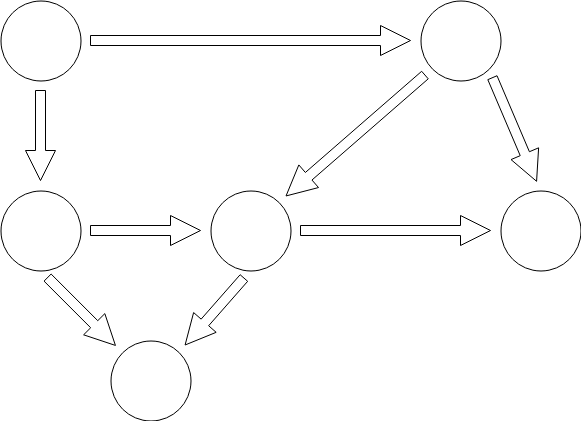
\includegraphics[width=.35\textwidth]{chapters/fig/assimetrico1.png}
\caption{Grafo Orientado ou Assimétrico}
\label{fig:assimetrico}
\end{figure}

Grafo não orientado ou simétrico - $G(V, E)$, $A = \emptyset$: uma aresta $(u,v)$ é dita não-orientada
se o par $(u,v)$ não for ordenado. As aresta não-orientadas são por vezes denotadas como conjunto ${u,v}$,
mas, para simplificar, é utilizado a notação de pares ordenados $(u,v)$, notando que no caso não-orientados
$(u,v)$ é o mesmo que $(v,u)$ \cite{goodrich}, figura \ref{fig:simetrico}.

\begin{figure}[htbp]
\centering
 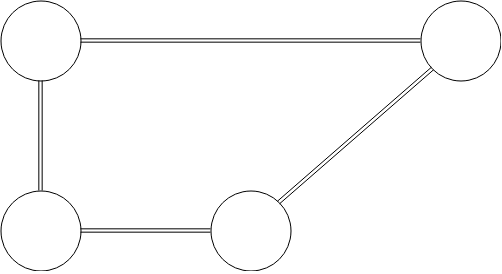
\includegraphics[width=.35\textwidth]{chapters/fig/simetrico1.png}
\caption{Grafo não Orientado ou Simétrico - $G(V,E)$}
\label{fig:simetrico}
\end{figure}
\FloatBarrier

Também é possível visualizar colaborações entre pesquisadores de certa área construindo um grafo cujos vértices são
associados aos pesquisadores e cujas arestas conectam pares de vértices associados aos pesquisadores
que escreveram juntos um artigo ou livro (Figura \ref{fig:goodrich}). Tais arestas são não-orientadas porque
a co-autoria é uma relação simétrica, ou seja, se A é co-autor de B, então necessariamente B é co-autor de A.

\begin{figure}[htbp]
\centering
 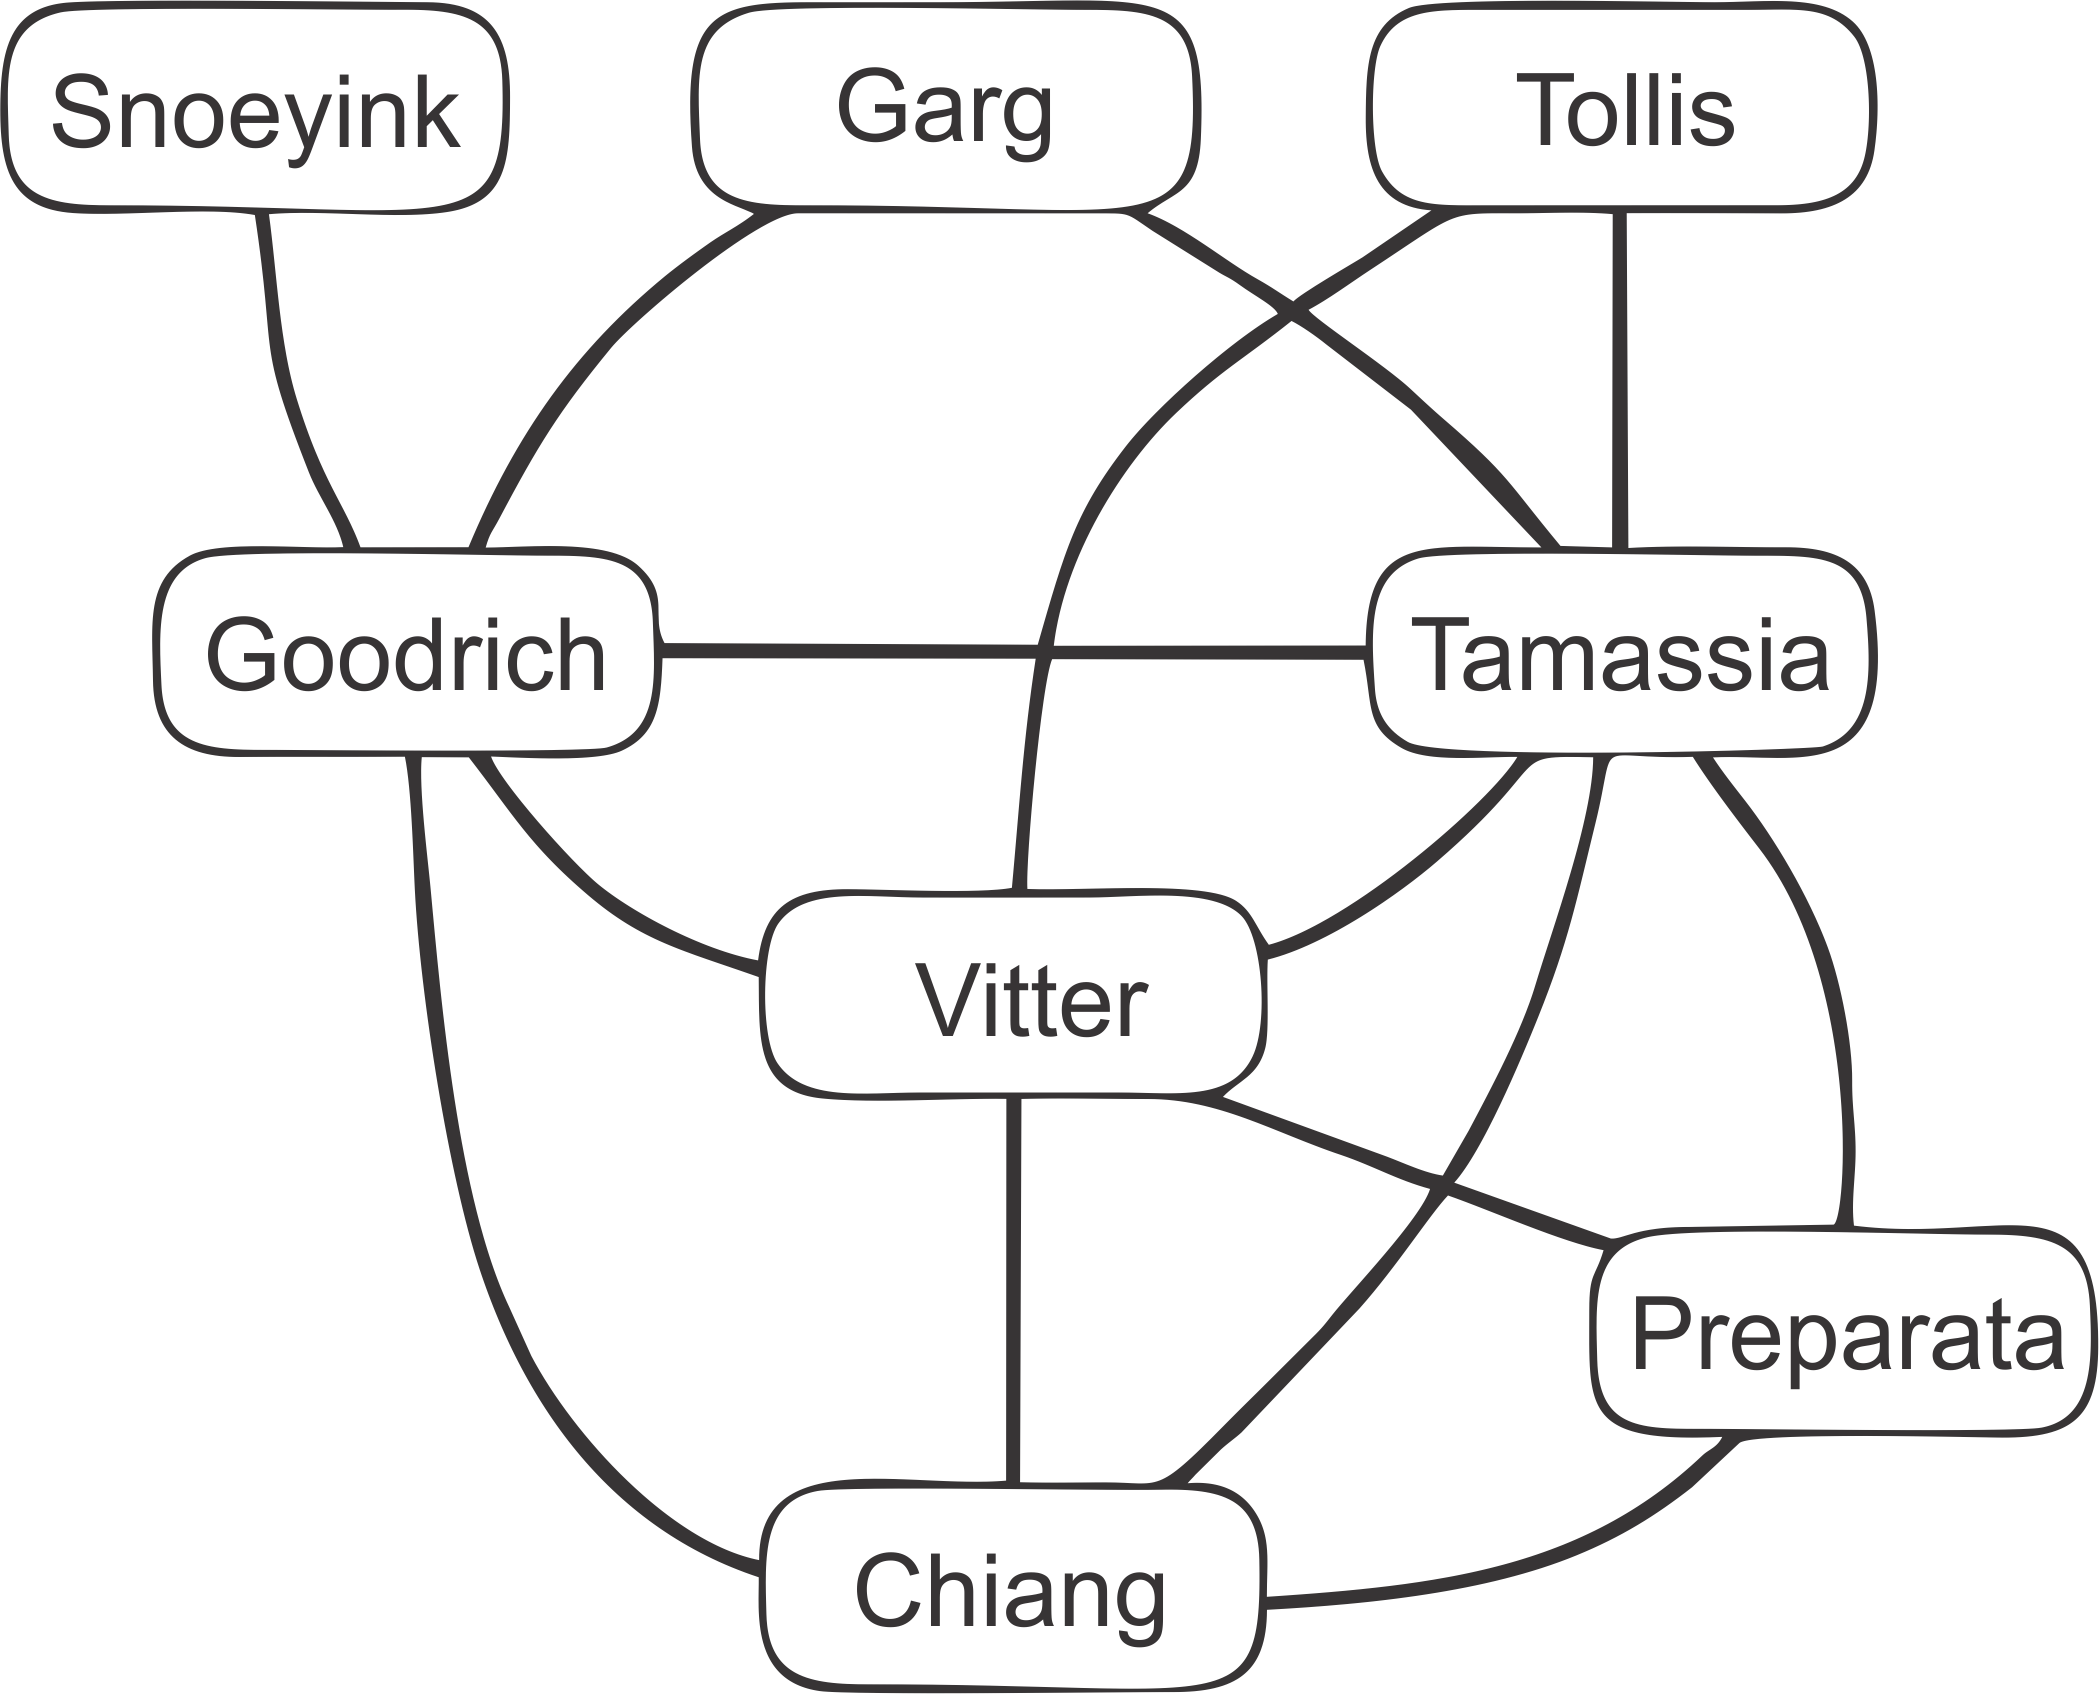
\includegraphics[width=.35\textwidth]{chapters/fig/goodrich.png}
\caption{Grafo de co-autoria de alguns autores}
Fonte: Elaboração própria, baseada em \cite{goodrich}
\label{fig:goodrich}
\end{figure}
\FloatBarrier


\cite{goodrich} diz que se todas as arestas em um grafo forem não-dirigidas,
então diz-se que o grafo é um grafo não-dirigido. De forma similar, um grafo dirigido, ou dígrafo, é um grafo em
que todas as arestas são dirigidas. Um grafo que tem arestas dirigidas e não-dirigidas é chamado de grafo misto, 
como mostra a figura \ref{fig:misto}.
Um mapa viário de uma cidade pode ser modelado como um grafo cujos vértices são cruzamentos ou finais de ruas, e cujas arestas
podem ser trechos de ruas sem cruzamentos. Este grafo tem arestas não-dirigidas, representando ruas de dois sentidos,
e arestas dirigidas, correspondendo a trechos de um único sentido. Assim, um grafo que representa as ruas de uma cidade
é um grafo misto.

\begin{figure}[htbp]
\centering
 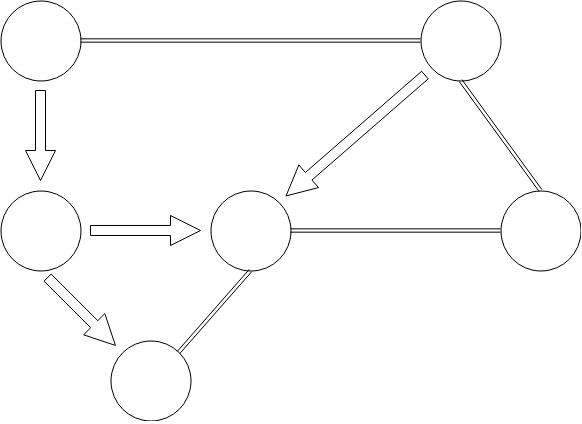
\includegraphics[width=.35\textwidth]{chapters/fig/misto1.png}
\caption{Grafo Misto - $G(V,E,A)$}
\label{fig:misto}
\end{figure}

\section{Rede de Topologia Estática}
Várias estruturas representam esse tipo de rede, como: estrutura matricial,
estrutura de listas encadeadas, estrutura de listas duplamente
encadeadas, dentre outras \cite{negreiros}.
Segundo \cite{cormen}, existem duas maneiras para representar um grafo $G = (V,E)$:
como uma coleção de listas de adjacências ou como uma matriz de adjacências. A representação
de lista de adjacências em geral é preferida, porque ela fornece um modo compacto para representar grafos esparsos,
onde para os quais $|E|$ é muito menor que $|V|^2$. Contudo, uma representação de matriz de adjacências pode ser
preferível, quando o grafo é denso, onde $|E|$ está próximo de $|V|^2$, ou quando é preciso ter a possibilidade
de saber com rapidez se existe uma aresta conectando dois vértices dados.

Segundo \cite{goldbarg}, uma matriz $A = |a_{ij}|$ quadrada de ordem $n$ é denominada matriz de adjacência de $G = (V, E)$ quando:\\
\indent $a_{ij}$ = 1, se $\exists(i,j)$ $\in$ $E$\\
\indent $a_{ij}$ = 0 em caso contrário.

As figuras \ref{fig:matriznaodirecionada} e \ref{fig:matrizdirecionada} apresentam exemplos de matrizes de adjacências para
grafos não direcionados e direcionados, respectivamente.

\begin{figure}[htbp]
\centering
 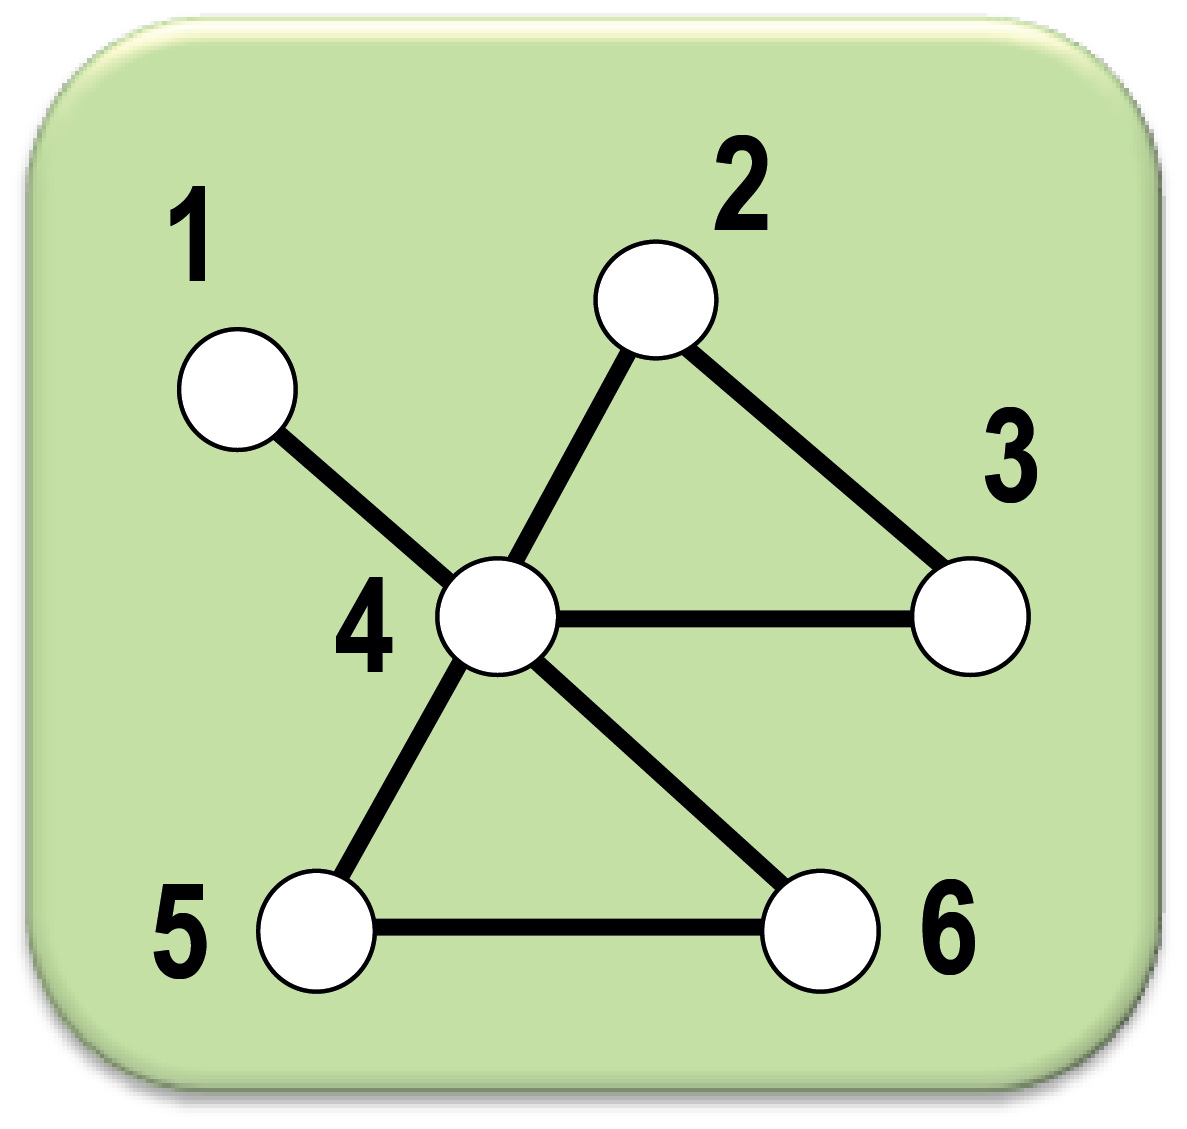
\includegraphics[width=.20\textwidth]{chapters/fig/cal_fig_091a.jpg}
 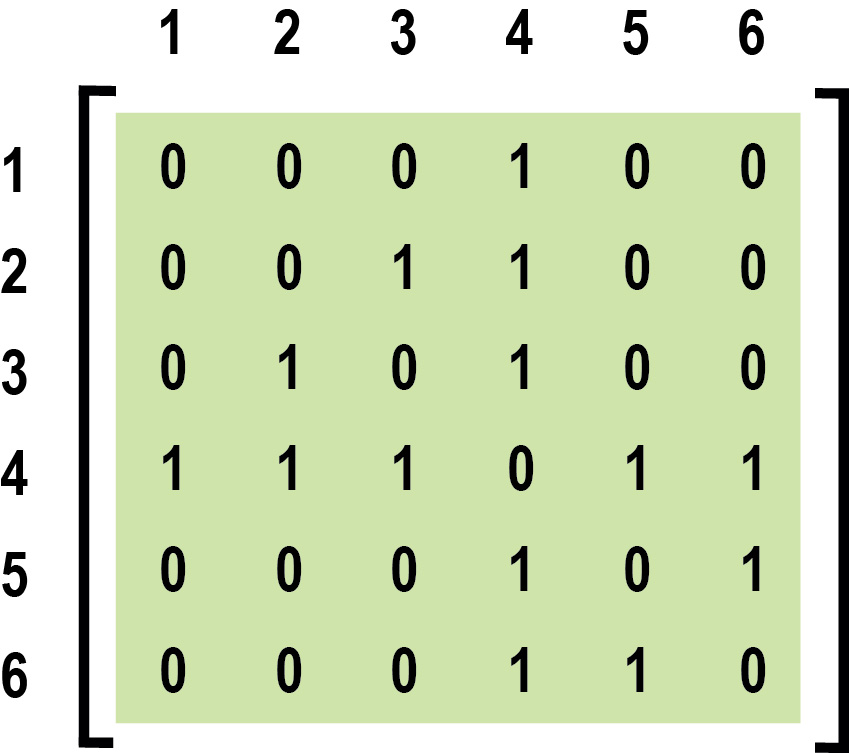
\includegraphics[width=.25\textwidth]{chapters/fig/cal_fig_091b.jpg}
\caption{Matriz de adjacências de grafo não direcionado}
Fonte: \cite{goldbarg}
\label{fig:matriznaodirecionada}
\end{figure}

\begin{figure}[htbp]
\centering
 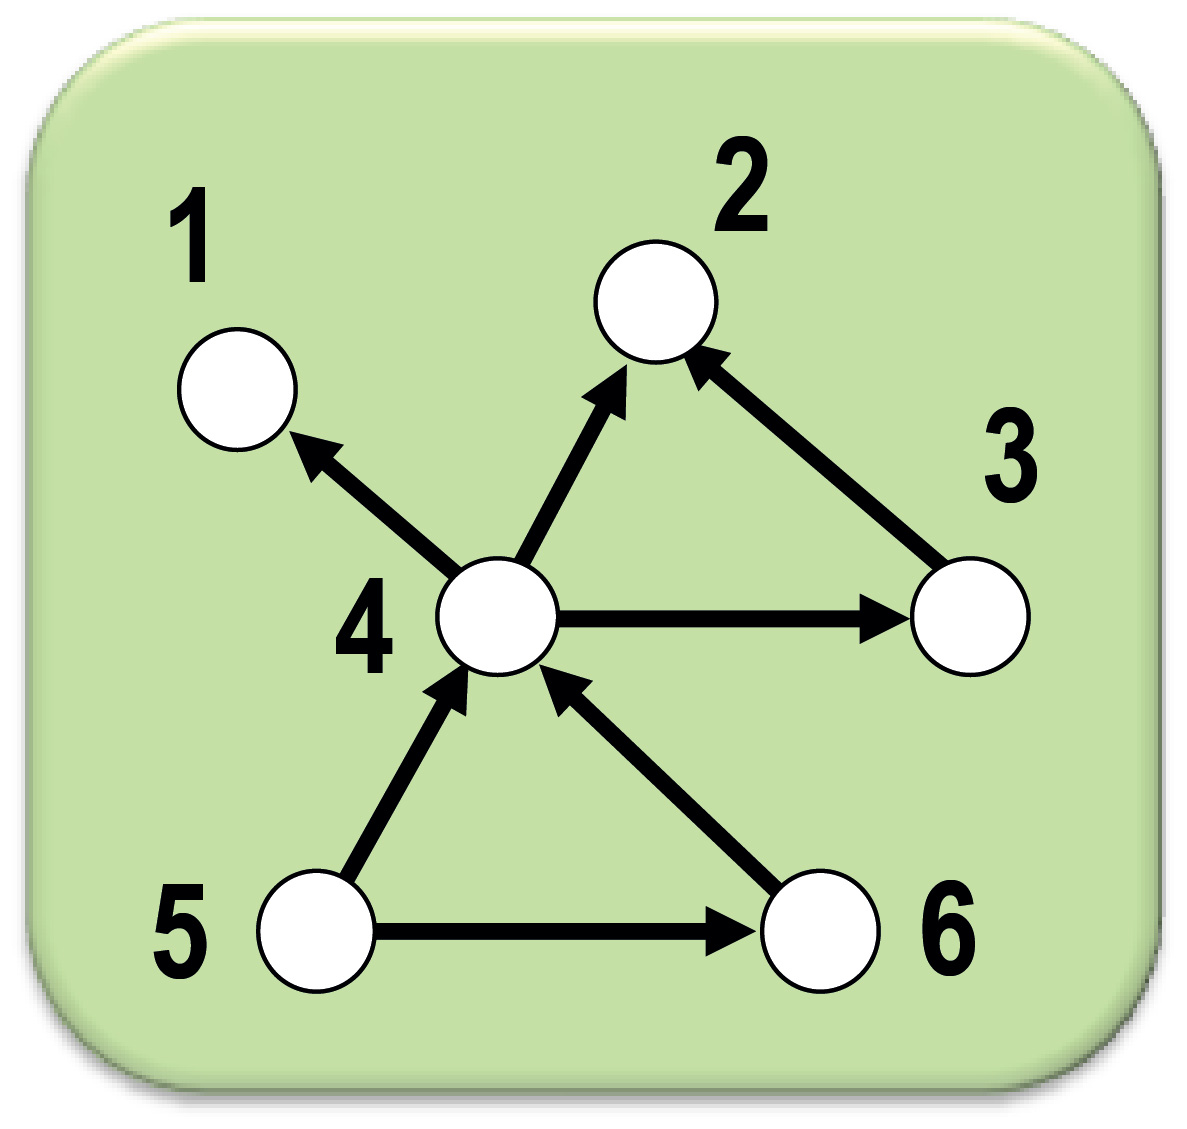
\includegraphics[width=.20\textwidth]{chapters/fig/cal_fig_092a.jpg}
 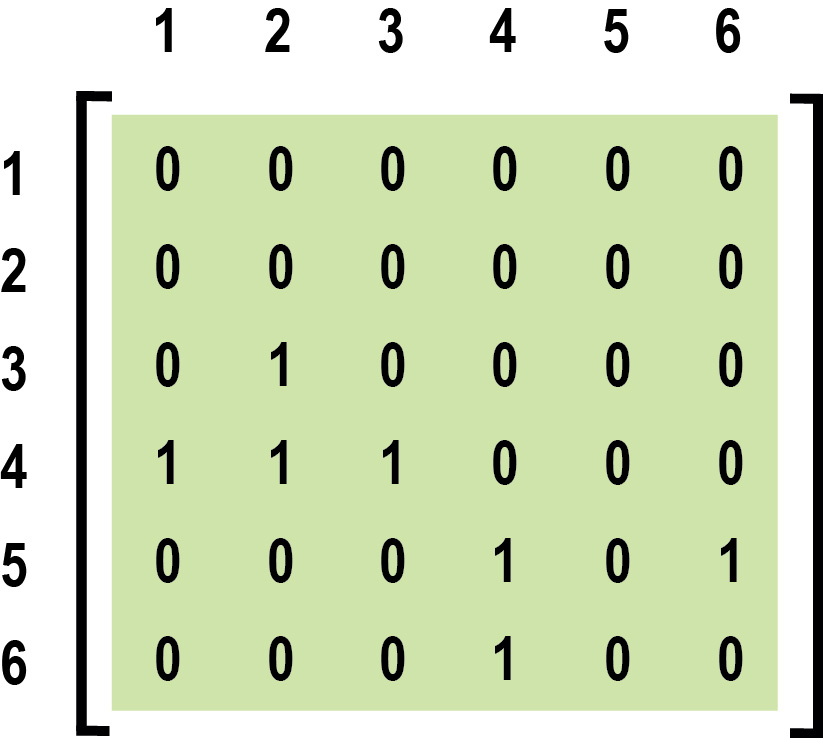
\includegraphics[width=.25\textwidth]{chapters/fig/cal_fig_092b.jpg}
\caption{Matriz de adjacência de grafo direcionado}
Fonte: \cite{goldbarg}
\label{fig:matrizdirecionada}
\end{figure}

Em Listas Encadeadas, segundo \cite{negreirosbook} e \cite{cormen}, quando se deseja armazenar um grafo pouco denso, ou seja,
$D_{max} \leqslant$ $\dfrac{|V|}{2}$ é mais vantajoso usar estruturas mais eficientes de armazenamento, assim como as listas
e vetores de listas. Neste caso, os vértices estão posicionados no vetor principal, onde a própria célula do vetor
guarda o rótulo do vértice que entrou primeiro e assim sucessivamente, como numa pilha. As pilhas, que derivam de cada
célula do vetor, podem ser construídas levando-se em conta as ligações de arcos/elos ao elemento vértice da célula
que o gera. No índice de cada célula de lista, mantém-se pelo menos uma informação contendo o vértice de ligação,
figura \ref{fig:listaencad}.
\FloatBarrier
\noindent $Type$\\
Lista: $\string^$ Lta;\\
$Lta$ = Record\\
$v$ : word; \{ Arco/elo ligado a VV\_i \}\\
$prx$ : Lista;\\
end;\\
$VV$ = Array[1..n] of Lista;\\

\begin{figure}[htbp]
\centering
 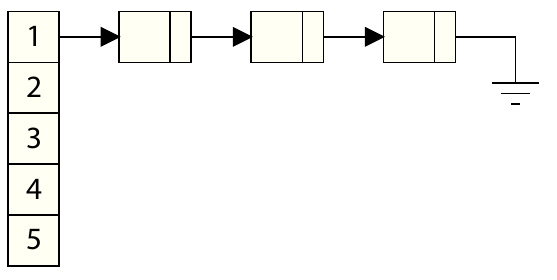
\includegraphics[width=.45\textwidth]{chapters/fig/listaencad.png}
\caption{Representação em Listas Encadeadas de um grafo}
Fonte: \cite{dynagraph} apud \cite{negreirosbook}
\label{fig:listaencad}
\end{figure}

Estruturas de Listas Duplamente Encadeadas são da forma, representada na figura \ref{fig:listdupla}, segundo \cite{negreirosbook}:
\FloatBarrier
\noindent $Type$\\
Lista: $\string^$ Lta;\\
$Lta$ = Record\\
$v$ : word; \{ Arco/elo ligado a VV\_i \}\\
$prx$ : Lista;\\
$ant$ : Lista;\\
end;\\
$VV$ = Array[1..n] of Lista;\\

\begin{figure}[htbp]
\centering
 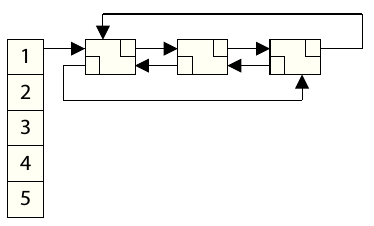
\includegraphics[width=.45\textwidth]{chapters/fig/listdupla.png}
\caption{Representação de um grafo em Listas Duplamente Encadeadas}
Fonte: \cite{dynagraph} apud \cite{negreirosbook}
\label{fig:listdupla}
\end{figure}

\FloatBarrier

\section{Redes Dinâmicas}

Em \cite{harary}, são definidas três tipos de redes: rede de nodos, rede de elos e rede ponderada.
\begin{itemize}
\item Uma rede de nodos (ou grafo de nodos ponderados) é uma tripla $(V, E, f)$, onde $V$ é um conjunto
de vértices, $E$ é um conjunto de arestas $\{u,v\}$, e $f$ é uma função, $f: V \rightarrow N$ onde $N$
é um sistema numérico, atribuição de um valor ou um peso.
\item Uma rede de elos (ou grafo de arestas ponderadas) é uma tripla $(V, E, g)$, definida de forma semelhante.
\item Uma rede ponderada (ou grafo totalmente ponderado) tem pesos atribuídos a ambos nós e arestas.
\end{itemize}

Outro tipo de rede é chamada de rede genérica, que contém atributos e características.

Grafo Dinâmico $G^t(V^t, L^t)$ é todo grafo que modifica seus vértices ($V^t$) e/ou ligações ($L^t$)
ao longo de um período de tempo ($H \in [T_i, T_k]$). Ou seja, as entidades $V$ (um conjunto de nodos),
$E$ (um conjunto de elos), $f$ (mapeamento de vértices para números) e $g$ (mapeamento de arestas para números)
podem se modificar dentro do intervalo H.
Logo, existem cinco tipos básicos de Grafos Dinâmicos.

\begin{itemize}
\item Em um grafo ou dígrafo com nós dinâmicos, o conjunto $V$ varia com o tempo. Assim, alguns nós podem
ser adicionados ou removidos. Quando os nós são removidos, as arestas ligadas a eles também são removidas; 
\item Em um grafo ou dígrafo com elos dinâmicos, o conjunto $E$ varia com o tempo. Assim, os arcos podem
ser adicionados ou removidos a partir do grafo ou dígrafo;
\item Em um grafo dinâmico de nodos ponderados, a função $f$ varia com o tempo. Assim, os pesos nos nós também variam;
\item Em um grafo dinâmico de elos ponderados, a função $g$ varia com o tempo;
\item Em um grafo dinâmico totalmente ponderado (ou grafo com topologia e atributos dinâmicos), ambas as funções $f$ e $g$
podem variar com o tempo.
\end{itemize}

\subsection{Topologia Estática e Atributos Dinâmicos}
Nesta rede os vértices e as arestas são constantes ao longo do tempo, mas seus atributos podem ser alterados.
O grafo é definido como $G(V^t, L^t)$, onde $V^t$ e $L^t$ são constantes no horizonte $H \in [T_i, T_k]$.
A figura \ref{fig:tead} exemplifica este grafo.

\begin{figure}[htbp]
\centering
 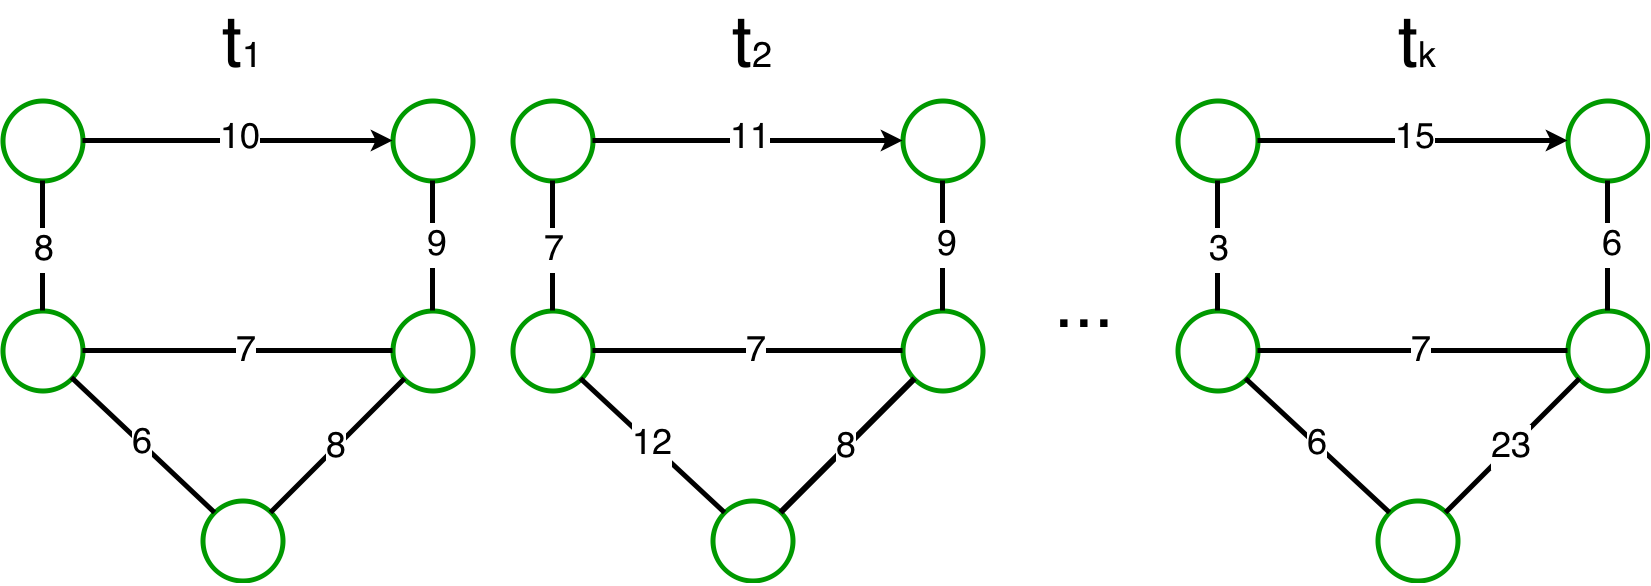
\includegraphics[width=.80\textwidth]{chapters/fig/tead.png}
\caption{Grafo com Topologia Estática e Atributos Dinâmicos}
\label{fig:tead}
\end{figure}

\subsection{Topologia Dinâmica e Atributos Estáticos}
\label{subsec:topdinatribest}
Nesta rede, ao longo do tempo, os vértices e as arestas podem ser removidos, adicionados e até mesmo
modificados para outra posição, mas suas características como espessura, cor e tamanho são fixas.
O grafo é definido como $G(V^t, L^t)$, onde $V^t$ e $L^t$ mudam no horizonte $H \in [T_i, T_k]$,
porém os atributos sempre serão os mesmos. A figura \ref{fig:tdae} mostra um exemplo desse grafo.

\begin{figure}[htbp]
\centering
 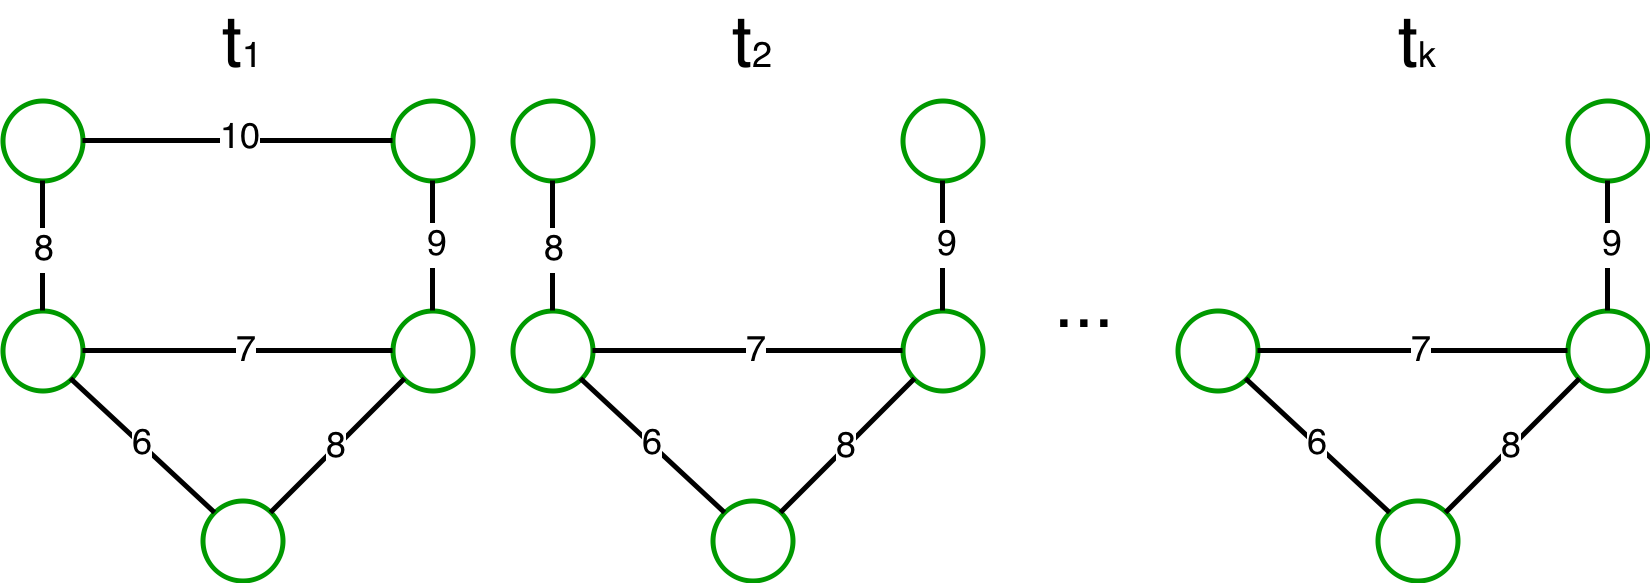
\includegraphics[width=.80\textwidth]{chapters/fig/tdae.png}
\caption{Grafo com Topologia Dinâmica e Atributos Estáticos}
\label{fig:tdae}
\end{figure}

\FloatBarrier

\subsection{Topologia e Atributos Dinâmicos}
\label{subsec:topdinatridin}
Nesta rede, o grafo é definido como $G(V^t, L^t)$, onde $V^t$ e $L^t$ mudam no horizonte $H \in [T_i, T_k]$, como
visto na figura \ref{fig:tdat}.
Estas redes são mais complexas \cite{dynagraph}, pois lidam com grande volume de dados comparadas as redes anteriores descritas.

\begin{figure}[htbp]
\centering
 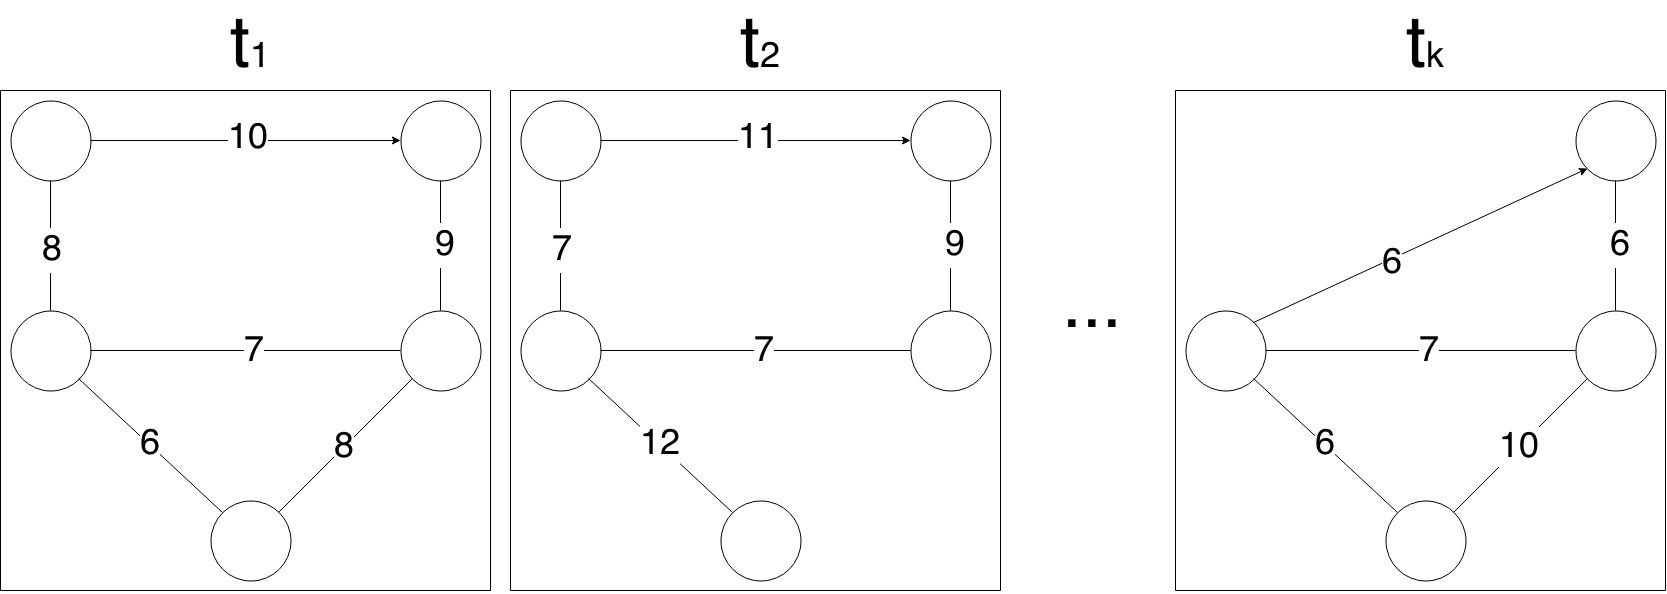
\includegraphics[width=.80\textwidth]{chapters/fig/tdat.png}
\caption{Grafo com Topologia e Atributos Dinâmicos}
\label{fig:tdat}
\end{figure}

\FloatBarrier

\section{Geração e manutenção de Redes Dinâmicas}
Os seguintes trabalhos abordam grafos dinâmicos e são utilizados como base deste trabalho:
\begin{itemize}
\item Modelo de Kim e Anderson, \cite{kim};
\item Gephi, \cite{gephi};
\item Dynagraph, \cite{dynagraph}.
\end{itemize}


\subsection{O modelo de Kim e Anderson}
A ideia central de \cite{kim} é modelar uma rede dinâmica como digrafos orientados
ao tempo (time-ordered graph), que é gerada através da ligação de instantes temporais com arestas
direcionadas que unem cada nó ao seu sucessor no tempo. Com isso, transformar uma rede dinâmica
em um grafo maior, mas facilmente analisável. Isto permite não só a utilização dos algoritmos
desenvolvidos para gráficos estáticos, mas também para melhor definir métricas para
gráficos dinâmicos.

Segundo \cite{kim} um sistema de grafos dinâmicos é um objeto de representação visual que pode descrever
melhor o comportamento dinâmico de objetos relacionados a eventos dinâmicos e introduzir
novas formas de enxergar ou descrever a evolução de eventos dinâmicos na natureza.

Assumindo que a duração de um período observado é finito, de um tempo inicial $t_{start}$ até o tempo final $t_{end}$, sem perda de
generalidade, é dado $t_{start}$ = $0$ e $t_{end}$ = $T$. Uma rede dinâmica $G^D_{0,T}$ = $(V, E_{0,T})$ consiste
em um conjunto de vértices e arestas temporais existentes no intervalo de tempo $[0,T]$, onde
os vértices $V$ e conjunto de arestas temporais $E_{0,T}$, onde uma aresta $(u,v)_{i,j}$ $\in$ $E_{0,T}$
existe entre vértices $u$ e $v$ em um intervalo de tempo $[i,j]$, tal que $i \leqslant T$ e $j \geqslant 0$ \cite{kim}.

Neste modelo, em uma rede dinâmica, o conjunto de vértices $V$ é sempre o mesmo, enquanto o conjunto de arestas existentes
muda ao longo do tempo.

A letra $w$ representa a duração de cada $snapshot$ (ou janela de tempo) e expressa em alguma unidade de tempo (como segundos ou horas).

Conforme \cite{kim}, uma rede dinâmica pode ser representada como uma série de grafos estáticos
$G_1, G_2, ..., G_N$. A notação $G_t(1 \leqslant t \leqslant n)$ representa o grafo agregado que consiste
de um conjunto de vértices $V$ e um conjunto de arestas $E_t$, onde uma aresta $(u,v)$ $\in$ $E_t$ existe
somente se uma aresta temporal $(u,v)_{i,j}$ $\in$ $E_{0,T}$ existe entre os vértices $v$ e $u$ no intervalo
de tempo $[i,j]$, tal que $i \leqslant wt$ e $j > w(t-1)$. $G_t$ é o t-ésimo $snapshot$ temporal de uma
rede dinâmica $G^D_{0,T}$ durante a t-ésima janela de tempo.

A tabela \ref{tab:kim} mostra uma relação de arestas e seus intervalos de existência. A figura \ref{fig:grafoKim} mostra os mesmos
dados desta tabela, em uma série de grafos estáticos e representação agredada.

\begin{table}[htbp]
	\centering
	\begin{tabular}{l l l l l l}
	\toprule
	\\Aresta & & & & & Intervalo de tempo\\
	\midrule
	\\(A,C) & & & & & [1,1]\\
	\\(A,D) & & & & & [2,2]\\
	\\(B,D) & & & & & [2,3]\\
	\\(C,D) & & & & & [3,3]\\
	\bottomrule
	\end{tabular}
\caption{Exemplo de contatos (arestas) em uma rede dinâmica}
 \label{tab:kim}
\end{table}

\begin{figure}[htbp]
\centering
 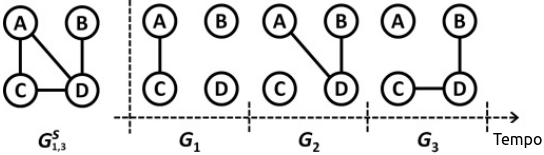
\includegraphics[width=.55\textwidth]{chapters/fig/kim.png}
\caption{Comparação entre a representação de grafos agregados(esquerda) e representação de sequência temporal(direita)}
Fonte: \cite{kim}
\label{fig:grafoKim}
\end{figure}
\FloatBarrier

\subsection{Gephi}
Gephi é um software de código aberto para análise e manipulação de redes.
Ele usa um motor de renderização 3D para exibir grandes redes em tempo real e para acelerar a exploração.
Módulos desenvolvidos podem importar, visualizar, espacializar, filtrar, manipular e exportar todos os tipos de redes \cite{gephi}.

Segundo \cite{dynagraph} o Gephi a princípio, seria um aplicativo para grafos estáticos, porém, posteriormente
foi incorporada uma característica temporal à sua estrutura. Seus dados são baseados em
uma espécie de matriz para vértices e uma outra para arestas. Cada coluna representa uma
informação. Para os vértices, há colunas como identificador, rótulo, posição, tamanho, cor
e intervalo de tempo. Para as arestas, há colunas para o identificador, origem, destino, o
tipo (dirigido ou não), rótulo, peso e cor. No modelo proposto, é possível adicionar novas
colunas para vértices ou arestas, e apenas nestas é possível definir informações que mudam
no tempo.

Como o Gephi não permite que alguns tipos de dados estruturados sejam modificados ao longo do tempo,
os vértices não podem mudar de posição no tempo, tampouco suas características visuais durante a sua existência.
O mesmo acontece com as mudanças de características visuais das arestas, que se mantêm constantes. Apesar
disto, os atributos dos vértices e arestas podem modificar no tempo \cite{dynagraph}.

As figuras \ref{fig:gephiUm} e \ref{fig:gephiDois} mostram a interface gráfica do Gephi.

\begin{figure}[htbp]
\centering
 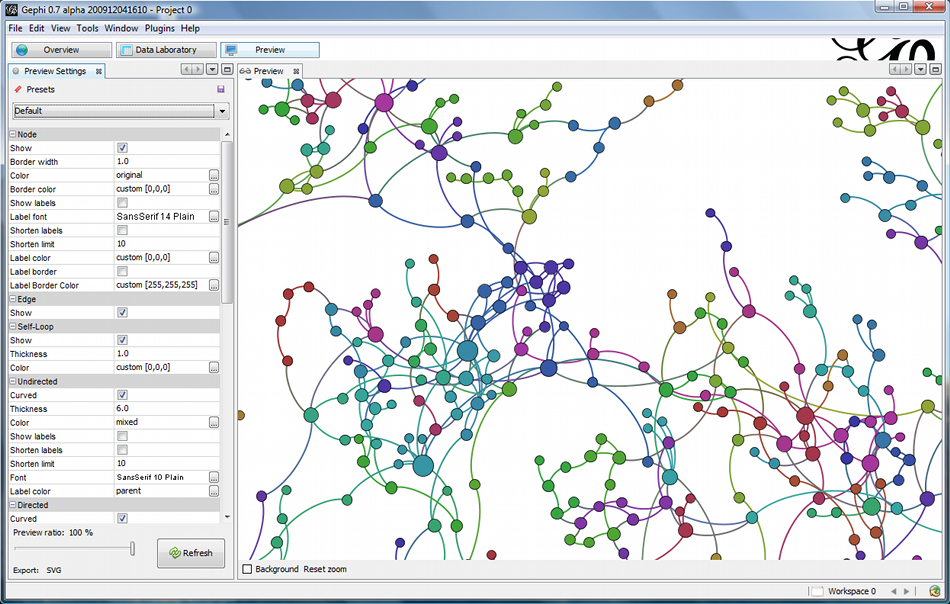
\includegraphics[width=.90\textwidth]{chapters/fig/gephiUm.png}
\caption{Captura de tela do software Gephi}
Fonte: gephi.github.io
\label{fig:gephiUm}
\end{figure}

\begin{figure}[htbp]
\centering
 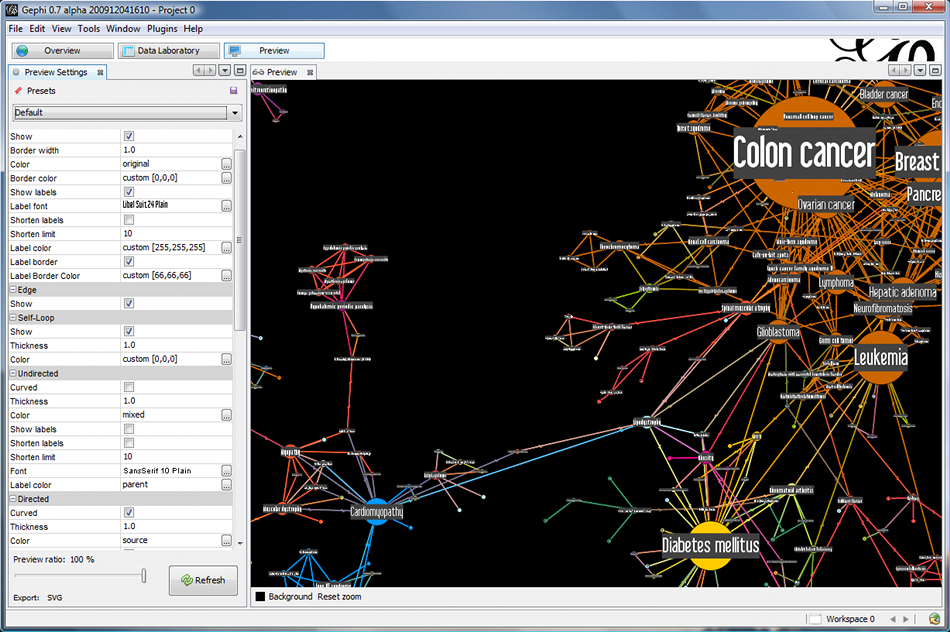
\includegraphics[width=.90\textwidth]{chapters/fig/gephiDois.png}
\caption{Captura de tela do software Gephi}
Fonte: gephi.github.io
\label{fig:gephiDois}
\end{figure}
\FloatBarrier

\pagebreak

\subsection{O modelo Dynagraph}
O modelo Dynagraph \cite{dynagraph} é baseado na primeira proposta em \cite{dynagraph2012}, que por sua vez é baseado no modelo
de \cite{kim}, porém o Dynagraph usa sequências temporais para vértices, arestas, características modificáveis dos vértices e arestas e
o relacionamento entre suas características. Com isso, é formado um grafo com as informações necessárias para qualquer instante no tempo.
O Dynagraph é capaz de visualizar o comportamento do grafo ao longo de um período de tempo, e editá-lo. A ferramenta construída permite
visualizar previsões e processos dinâmicos em vários contextos e realizar simulações preditivas sobre estes eventos \cite{dynagraph}.

Um grafo dinâmico é definido por $G^t$, que ocorre no intervalo $t = [t_s,t_f]$, onde $t_s$ é o tempo inicial e $t_f$ é o tempo final.
$G^t = (V^{t_v}, E^{t_e})$, onde $t_v \subseteq t$ e $t_e \subseteq t$, e $V^{t_v}$ e $E^{t_e}$ são funções que geram vértices e arestas
respectivamente, em função do intervalo $t=t_v \cup t_e$.

As estruturas $V^{t_v} = \{O^{t_v}, F^{t_v}\}$ para vértices e $E^{t_e} = \{O^{t_e}, F^{t_e}\}$ para arestas são semelhantes,
onde $O^{t_v} = \{O_{0_v}, O_{1_v},..., O_{i_v}\}$ e $O^{t_e} = \{O_{0_e}, O_{1_e},..., O_{i_e}\}$ os objetos indexados de objetos,
e $F^{t_v} = \{F^{t_v}_{0_v}, F^{t_v}_{1_v},..., F^{t_v}_{w_v}\}$ e $F^{t_e} = \{F^{t_e}_{0_e}, F^{t_e}_{1_e},..., F^{t_e}_{w_e}\}$ os
conjuntos indexados de características modificáveis destes objetos \cite{dynagraph}.

A estrutura de dados usada no Dynagraph segue a Notação de Objeto Javascript (JSON), que é um formato de texto de intercâmbio de dados \cite{douglas}.
A figura \ref{fig:jsondyn} mostra como é essa estrutura seguindo três objetos principais: ``metadata'', ``binding'' e ``data''.

Em ``metadata'' são definidos os campos para utilização de qualquer identificador, por exemplo é possível utilizar ``ini'' e ``fim'',
que representam o tempo inicial e final de um elemento, no lugar de ``start'' e ``end'' respectivamente.

Em ``binding'' são definidas as características dos vértices e arestas. Seguindo o exemplo da figura \ref{fig:jsondyn}, ``vertex'' poderá
ser do tipo ``v1'', ``v2'' e ``v3'', onde cada tipo contém informações da forma do vértice. Essa forma pode ser uma imagem no formato
``png'' ou ``jpg'' ou customizada com as seguintes características:
\begin{itemize}
\item path: círculo ou seta;
\item fillColor: cor do preenchimento;
\item strokeColor: cor da borda;
\item fillOpacity: opacidade;
\item scale: tamanho;
\item strokeWeight: espessura da borda.
\end{itemize}
A aresta, ou ``polyline'', segue uma estrutura semelhante a do ``vertex'', porém com algumas particularidades como repetição de um símbolo
ao longo da aresta, e uma customização no campo ``path'' seguindo a notação
SVG\footnote{\label{note} Scalable Vector Graphics - é uma forma de descrever de forma vetorial desenhos e gráficos bidimensionais}.

Em ``data'' são definidos os elementos do grafo, os tempos de início e fim de cada elemento ou tempo de existência.
No caso dos vértices, a posição de cada elemento pode ser escrita no formato UTM ou latitude e longitude.
O tipo de cada elemento, descrito em ``binding'', e no caso das arestas, são definidos os pontos de origem e destino.

Na figura \ref{fig:jsondyn} vemos a estrutura de construção de um grafo dinâmico.
Os campos ``metadata'' e ``binding'' foram omitidos para evidenciar o objeto ``data''.
\FloatBarrier
\begin{center}
  \line(1,0){450}
\end{center}
\lstinputlisting[language=Java]{chapters/new.json}
\begin{figure}[htbp]
  \begin{center}
    \line(1,0){450}
  \end{center}
  \centering
  \caption{Estrutura JSON usada pelo Dynagraph}
  \label{fig:jsondyn}
\end{figure}

A figura \ref{fig:dynagraph} demonstra os dados do código da figura \ref{fig:jsondyn} sendo utilizados no software
Dynagraph com variações temporais no grafo e nas características de seus vértices e arestas.

\FloatBarrier
\begin{figure}[htbp]
\centering
 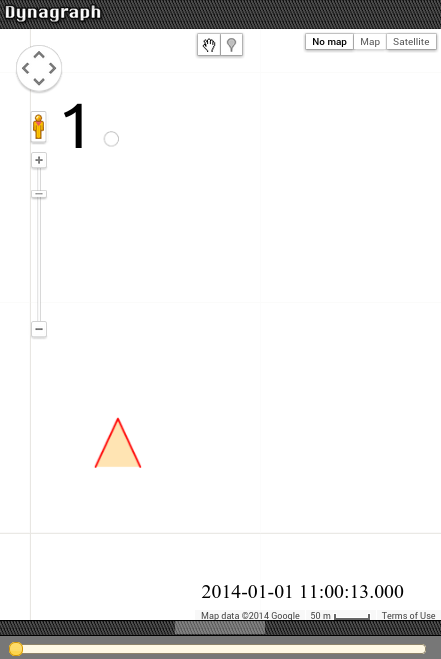
\includegraphics[width=.24\textwidth]{chapters/fig/b1mod.png}
 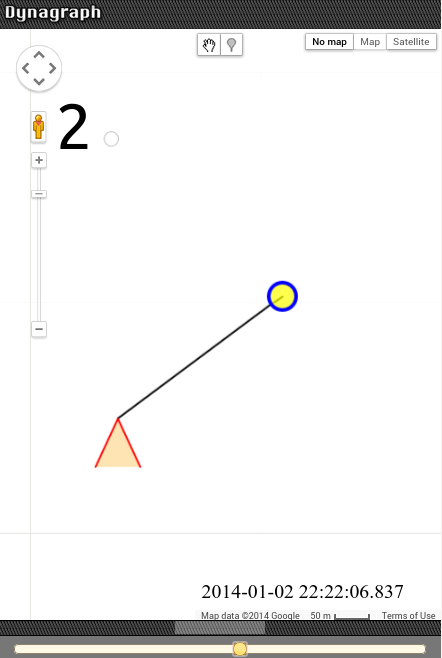
\includegraphics[width=.24\textwidth]{chapters/fig/b2mod.png}
 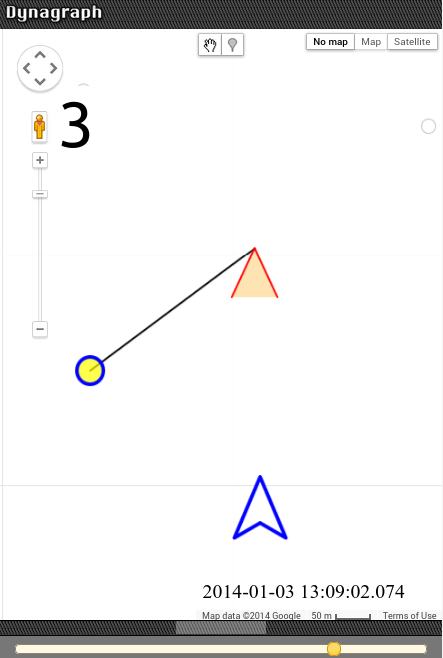
\includegraphics[width=.24\textwidth]{chapters/fig/b3mod.png}
 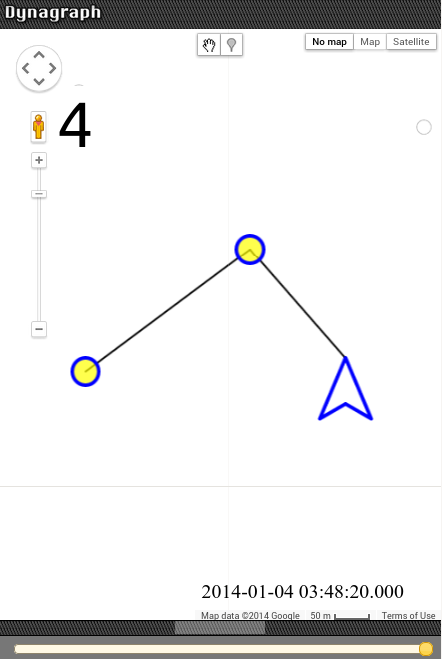
\includegraphics[width=.24\textwidth]{chapters/fig/b4mod.png}
\caption{Capturas de tela do software Dynagraph}
\label{fig:dynagraph}
\end{figure}


\chapter{Fundamentação Teórica}

\section{Caminhos em Redes Estáticas}
Dentre os diversos problemas que surgem em grafos, este é o mais fundamental de todos e
aquele que ao longo dos anos foi dos mais estudados. Várias técnicas surgiram desde os meados
de 1950 com o objetivo de tratar eficientemente o problema de caminhos mínimos em grafos. A
principal delas considera o fato de se promover uma arborescência em um grafo onde a medida
que os vértices explorados são atingidos, tem-se uma proximidade da solução do problema \cite{negreirosbook}.

\subsection{Problema de Caminho Mínimo}
Uma rede de transporte (que pode ser uma malha viária, rodoviária, etc.) pode ser
representada por uma grafo $G = (N, A)$, onde $N$ é o conjunto de nós e A é o conjunto de arcos
os quais interligam estes nós. Considerado o número de nós $|N| = n$ e o número de arcos $|A| = m;$ para
cada arco $(i, j) \in A$ está associado um custo unitário $c_{ij}$. O caminho entre um
nó origem $(s)$ e um nó destino $(t)$ é definido por uma sequência de
arcos: $(s,i),...(k,l),...(j,t)$. O Problema de Caminho Mínimo (PCM) consiste em determinar
um caminho entre $s$ e $t$ tal que a somatória dos custos unitários dos arcos (ou alguma
outra medida de impedância) que compõem este caminho seja o mínimo \cite{cunha}.

Dada uma rede $G$ com $m$ nós e $n$ arcos, associando a cada arco $(i,j)$ o custo $c_{ij}$, o Problema
de Caminho Mínimo é encontrar o menor caminho entre o nó 1 para o nó $m$ em $G$ (caminho mínimo de menor valor).
O custo do caminho é a soma dos custos sobre os arcos do caminho encontrado. Uma formatação genérica do problema
de caminho mínimo é dada via grafos, quando deseja-se encontrar o percurso de custo mínimo entre dois vértices $i$ e $j$
de um grafo $G(V,L)$, onde, se $\exists$ $\Gamma (i,j)$, $i$, $j \in V$, então $w_{ij}$ é tomado como o custo mínimo
de um caminho direto entre os vértices $i$ e $j$, e todo $i_1$, ..., $i_k \in V$, distintos de $i$, $j$, são ditos
serem vértices do caminho, onde $i$ precede $i_1$ e assim por diante, nesta ordem \cite{negreirosbook}.

\subsection{Algoritmo de Dijkstra}
O algoritmo de Dijkstra foi proposto em 1959 e permite determinar a solução ótima através da adição de
vértices à árvore de caminho mínimo pelo processo de relaxamento de uma aresta, que consiste em verificar
se há a possibilidade de melhorar o caminho obtido até o momento \cite{boaventura}. Este algoritmo considera
basicamente um processo de rotulação de vértices à medida que o mínimo caminho é encontrado passo a passo,
interativamente, em vértices intermediários. O algoritmo requer que nenhum peso no grafo seja negativo. Abaixo
é apresentado o pseudocódigo do algoritmo de Dijkstra segundo \cite{cormen}.

\fbox{\begin{minipage}{70ex}
\noindent \phantom{} \hspace{0ex} {\bf AlgoritmoDijkstra}\\
\vspace*{-1mm} \phantom{} \hspace{3ex} inicialize a distância para todos os nós em G = infinito\\
\vspace*{-1mm} \phantom{} \hspace{3ex} {\bf Para} inicialize o predecessor de todos os nós em G = vazio\\
\vspace*{-1mm} \phantom{} \hspace{3ex} {\bf Enquanto} H não estiver vazio faça\\
\vspace*{-1mm} \phantom{} \hspace{6ex} u = o nó com menor rótulo extraído de H\\
\vspace*{-1mm} \phantom{} \hspace{6ex} {\bf Para} cada v adjacente a u:\\
\vspace*{-1mm} \phantom{} \hspace{9ex} {\bf Se} rótulo[v] > rótulo[u] + distância[u, v]:\\
\vspace*{-1mm} \phantom{} \hspace{12ex} rótulo[v] = rótulo[u] + distância[u, v];\\
\vspace*{-1mm} \phantom{} \hspace{12ex} predecessor[v] = u;\\
\vspace*{-1mm} \phantom{} \hspace{12ex} atualiza a posição de v em H\\
\vspace*{-1mm} \phantom{} \hspace{9ex} {\bf Fim Se}\\
\vspace*{-1mm} \phantom{} \hspace{6ex} {\bf Fim Para}\\
\vspace*{-1mm} \phantom{} \hspace{3ex} {\bf Fim Enquanto}\\
\vspace*{-1mm} \phantom{} \hspace{0ex} {\bf Fim Dijkstra}\\
\end{minipage}}

\subsection{Algoritmo Radix Heap}
O algoritmo Radix Heap é utilizado numa variação do algoritmo de Dijkstra e foi proposto inicialmente por
Ahuja, Mehlhorn, Orlin e Tarjan em \cite{ahuja}.
Ele é considerado ainda no meio científico como um dos algoritmos mais eficientes para resolver o
problema do caminho mínimo.
A implementação do Radix Heap é um híbrido da implementação primitiva $O(n^2)$ e implementação de Dial($O(m + nC))$). 
Estas duas implementações representam dois extremos no que diz respeito à quantidade dos buckets utilizados.
A implementação primitiva considera todos os vértices rotulados temporariamente juntos, em um bucket grande,
e procura por um vértice com o menor rótulo. Já o algoritmo de Dial usa um grande número de buckets e separa os vértices,
armazenando dois vértices quaisquer com rótulos diferentes em diferentes segmentos \cite{bookahuja}.
A implementação Radix Heap melhora esses dois métodos através de uma solução intermediária:
Ele armazena vários, mas não todos os vértices em um mesmo bucket. Por exemplo, em vez de armazenar
apenas os vértices com $d[v] = k$ em um bucket k, como na implementação do Dial,
pode-se armazenar todos os vértices com $d[v]$ dentro do intervalo [100$k$ para 100$k$ + 99] no bucket $k$ \cite{bookahuja}.

Para o bucket[k] é definido um intervalo de valores denotado por intervalo(k). O número de inteiros
no intervalo é chamado de largura do intervalo e denotado por largura(k).
No exemplo anterior, o intervalo do bucket $k$ é [100$k$, 100$k$ + 99] e sua largura é de 100. 

Usando larguras de tamanho $k$ permite reduzir o número de buckets necessários por um fator de $k$.
Mas para encontrar o rótulo de menor distância, é preciso procurar todos os elementos no bucket não vazio de menor índice.
Para superar isso, o algoritmo radix heap considera usar larguras variáveis e altera os intervalos de forma dinâmica. 
O Radix Heap segue as propriedades:

1. As larguras dos buckets são 1, 1, 2, 4, 8, 16, ..., de modo que o número de buckets necessários é somente $O(log(NC))$.

2.  Os intervalos dos buckets são modificados dinamicamente e são realocados os vértices de menor rótulo temporário
para um único bucket, cuja largura é 1.

A Propriedade 1 nos permite manter apenas $O(log(NC))$ buckets e, assim, supera a desvantagem do algoritmo
de Dial, que usa muitos buckets.
A Propriedade 2 nos permite, como no algoritmo Dial, evitar a necessidade de 
pesquisar todo o bucket para encontrar um vértice de menor rótulo temporário. Quando implementado deste modo, esta 
versão do algoritmo radix heap tem complexidade $O(m + nlog(nC))$ \cite{bookahuja}.

Para um dado problema de caminho mínimo, o radix heap consiste em $1 + [log(NC)]$ buckets.
Os buckets são numeradas de $0$ até $K = [log(nC)]$.
O algoritmo irá alterar os intervalos dos buckets de forma dinâmica, e cada vez que muda os intervalos,
redistribui os vértices nos buckets. Inicialmente, os buckets têm os seguintes intervalos:\\
intervalo(0) = [0];\\
intervalo(1) = [1];\\
intervalo(2) = [2, 3];\\
intervalo(3) = [4, 7];\\
intervalo(4) = [8, 15];\\
...\\
intervalo(K) = [$2^{K - 1}$, $2^K - 1$].

Esses intervalos mudam à medida que o algoritmo prossegue. No entanto, a largura dos buckets nunca aumentam
para além das suas larguras iniciais \cite{bookahuja}.

\subsubsection{Operações sobre o Radix Heap}
Determinar qual intervalo contém um dado valor pode ser feito percorrendo o vetor de buckets com complexidade $O(lognC)$.
Logo, inserir um vértice na estrutura, tem complexidade $O(K)$, pois $O(K) = O(lognC)$

A operação que diminui a chave de um elemento $v$ é executada da seguinte forma: no tempo $O(K)$ determina-se
o bucket k tal que $d[v] \in intervalo(k)$. Logo após diminuir $d[v]$ basta determinar o novo bucket que vai conter
$v$, que pode ser feito em tempo $O(K)$.

Para descrever a operação de retirar o item da fila de prioridades que contém o menor valor chave considere o seguinte exemplo:
Supondo que o rótulo temporário de um vértice de conteudo(4) é 9, cujo intervalo é [8, 15].
O algoritmo irá examinar cada vértice em conteudo(4) para identificar um vértice com o rótulo de menor distância.
Segundo \cite{bookahuja}, os rótulos de distância que o algoritmo de Dijkstra designa como permanente não são decrescentes,
isso implica que nenhum rótulo temporário de distância jamais voltará
a ser inferior a 9 e, conseqüentemente, não precisará mais dos buckets de 0 a 3.

Em vez de deixar estes buckets inativos, o algoritmo redistribui o intervalo[9, 15]
para os buckets anteriores, resultando nos intervalos intervalo(0) = [9], intervalo(1) = [10],
intervalo(2) = [11, 12], intervalo(3) = [13,15] e intervalo(4) = $\emptyset$ . Uma vez que o intervalo(4)
está vazio agora, o algoritmo redistribui os vértices que estavam em conteudo(4) para os buckets adequados (0, 1, 2, e 3).
Assim, cada um dos vértices no bucket 4 move-se para um bucket de menor índice e todos vértices com o rótulo de menor distância
é movido para o bucket 0, que tem largura 1 \cite{bookahuja}.

\subsubsection{Funcionamento do Algoritmo de Dijkstra com Radix Heap}
Sempre que o algoritmo encontra vértices com o rótulo de menor distância em um bucket com
largura maior que 1, ele verifica todos os vértices no bucket para identificar um vértice com rótulo de menor distância.
Em seguida, o algoritmo redistribui o intervalo dos buckets e muda cada vértice no bucket para o bucket de menor índice.
Uma vez que o radix heap contém $k$ buckets, um vértice pode mudar na maioria das $k$ vezes, e consequentemente,
o algoritmo irá verificar qualquer vértice na maioria das $k$ vezes. Por isso, o número total de verificações
de vértices é $O(NK)$, o qual não é "muito grande" \cite{bookahuja}.

Para demonstrado o funcionamento do algoritmo de Dijkstra com Radix Heap serão utilizadas figuras do livro \cite{bookahuja}.
O grafo na Figura \ref{fig:grafoRadix} exemplifica o radix heap, e o número ao lado de cada arco indica o seu comprimento.
\FloatBarrier
\begin{figure}[htbp]
\centering
 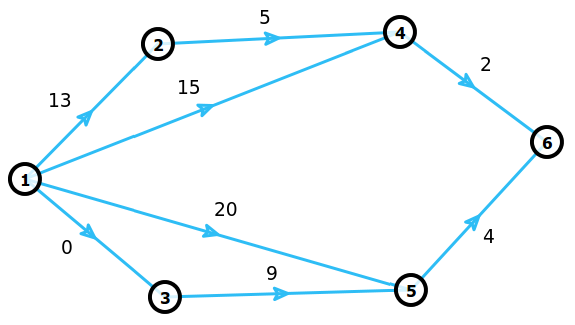
\includegraphics[width=.65\textwidth]{chapters/fig/grafoRadix.png}
\caption{Grafo - Caminho Mínimo}
\label{fig:grafoRadix}
\end{figure}
\FloatBarrier
O vértice origem é $s = 1$. O peso da maior aresta é $C = 20$, logo $K = [log(nC))] = [log(120)] = 7$.
A Tabela \ref{tab:initialradixheap} especifica os rótulos distância determinada pelo algoritmo de Dijkstra
após análise do vértice 1.
\FloatBarrier
\begin{table}[htbp]
	\centering
	\begin{tabular}{l l l l l l l}
	\toprule
	vértice $i$ & 1 & 2 & 3 & 4 & 5 & 6\\
	\midrule
	rótulo d[$i$] & 0 & 13 & 0 & 15 & 20 & $\infty$ \\
	\bottomrule
	\end{tabular}
	
	\centering
	\begin{tabular}{l l l l l l l l l}
	\toprule
	\\bucket $k$ & 0 & 1 & 2 & 3 & 4 & 5 & 6 & 7\\
	\midrule
	\\intervalo($k$) & [0] & [1] & [2, 3] & [4, 7] & [8, 15] & [16, 31] & [32, 63] & [64, 127]\\
	\\conteudo($k$) & \{3\} & $\emptyset$ & $\emptyset$ & $\emptyset$ & \{2, 4\} & \{5\} & $\emptyset$ & \\
	\bottomrule
	\end{tabular}
\caption{Radix Heap inicial}
 \label{tab:initialradixheap}
\end{table}

Para selecionar o vértice com o rótulo de menor distância, os buckets 0, 1, 2, ..., K são varridos para encontrar o
primeiro bucket não vazio. No exemplo, o bucket 0 é não vazio. Uma vez que o bucket 0 tem largura 1,
cada vértice neste bucket tem o mesmo (no mínimo) rótulo de distância. Assim, o algoritmo determina o vértice 3 como permanente,
exclui o vértice 3 do radix heap, e verifica o arco (3, 5) para alterar o rótulo de distância do vértice 5 de 20 para 9.
Em seguida, é verificado se o novo rótulo de distância do vértice 5 está contido no intervalo de seu bucket presente,
que é o bucket 5. Como o seu rótulo de distância diminuiu, o vértice 5 deve se mover para um bucket de menor índice.
Assim, é concluída a análise sequencial dos bucket da direita para a esquerda, a partir do bucket 5,
para identificar o primeiro bucket cujo intervalo contém o número 9, que é o bucket 4.
O vértice 5 é movido do bucket 5 para bucket 4. A tabela \ref{tab:secondradixheap} mostra o novo radix heap.

\begin{table}[htbp]
	\centering
	\begin{tabular}{l l l l l}
	\toprule
	vértice $i$ & 2 & 4 & 5 & 6\\
	\midrule
	rótulo d[$i$] & 13 & 15 & 9 & $\infty$ \\
	\bottomrule
	\end{tabular}
	
	\centering
	\begin{tabular}{l l l l l l l l l}
	\toprule
	\\bucket $k$ & 0 & 1 & 2 & 3 & 4 & 5 & 6 & 7\\
	\midrule
	\\intervalo($k$) & [0] & [1] & [2, 3] & [4, 7] & [8, 15] & [16, 31] & [32, 63] & [64, 127]\\
	\\conteudo($k$) & $\emptyset$ & $\emptyset$ & $\emptyset$ & $\emptyset$ & \{2, 4, 5\} & $\emptyset$ & $\emptyset$ & $\emptyset$\\
	\bottomrule
	\end{tabular}
\caption{Radix Heap - final da iteração 1}
 \label{tab:secondradixheap}
\end{table}
\FloatBarrier
Varrendo os buckets sequencialmente, é observado que o bucket $k = 4$ é o primeiro bucket não vazio.
Uma vez que o intervalo deste bucket contém mais de um número inteiro, o primeiro vértice no bucket não precisa ter
o rótulo de menor distância. Tem-se que intervalo(4) é [8, 15], mas como seu menor rótulo temporário neste bucket é 9,
o novo intervalo a ser redistribuído é intervalo[9, 15] da seguinte maneira:\\
intervalo(0) = [9],\\
intervalo(1) = [10],\\
intervalo(2) = [11, 12],\\
intervalo(3) = [13, 15],\\
intervalo(4) = $\emptyset$.

Outros intervalos não mudam. Os vértices do bucket 4 foram redistribuídos nos buckets 0 a 3.
Os buckets resultantes têm os seguintes conteúdo:\\
conteúdo(0) = {5},\\
conteúdo(1) = $\emptyset$,\\
conteúdo(2) = $\emptyset$,\\
conteúdo(3) = {2, 4},\\
conteúdo(4) = $\emptyset$.

Esta redistribuição esvazia necessariamente o bucket 4 e move o vértice com o rótulo de menor distância para o bucket 0.

\subsubsection{Complexidade do Algoritmo de Dijkstra com Radix Heap}
Cada operação de inserção do vértice no bucket consome tempo $O(K)$.
Como um vértice só pode ser movido $K$ vezes no máximo, então $O(nK)$ é um limite para o número total de movimentos
de vértices.
O termo $m$ significa o número de distâncias atualizadas, logo o tempo total gasto em atualizar os rótulos temporários
é $O(m + nK)$.
A operação de selecionar um vértice começa verificando os buckets da esquerda para a direita para encontrar
o primeiro bucket não vazio $k$ no radix heap. Esta operação requer tempo $O(K)$ por iteração e $O(nk)$ no total.
A redistribuição do intervalo segue atribuindo o primeiro inteiro para bucket 0, o próximo inteiro para bucket 1,
os próximos dois inteiros para bucket 2, nos próximos quatro inteiros para bucket 3, e assim por diante.
Uma vez que o bucket $k$ tem uma largura inferior a $2^{k - 1}$, e uma vez que as larguras dos primeiros $k$ buckets
pode ser tão grande como $1, 1, 2, ..., 2^{k - 2}$ até uma largura total de potencial $2^{k - 1}$,
o intervalo útil do bucket k sobre os buckets $0, 1, ..., k - 1$ é redistribuido.
Esta redistribuição dos intevalos e re-inserções subsequentes de vértices esvazia o bucket k e move os vértices com
os rótulos de menor distância para o bucket 0 \cite{bookahuja}.
Portanto, como $k = [log(nC)]$, o tempo de execução do algoritmo de Dijkstra com Radix Heap é $O(m + nk) = O(m + n log(nC))$.
Usando a estrutura de dados Fibonacci heap com a implementação do radix heap, é possível reduzir ainda mais a complexidade
para $O(m + n\sqrt{logC})$, o que dá uma execução mais rápida do algoritmo em tempo polinomial para resolver
o problema do caminho mínimo com comprimentos de arcos não negativos \cite{ahuja}.
A Figura \ref{fig:codeRadix} apresenta o pseudocódigo do algoritmo Radix Heap.

\fbox{\begin{minipage}{70ex}
\noindent \phantom{} \hspace{0ex} {\bf AlgoritmoRadixHeap}\\
\vspace*{-1mm} \phantom{} \hspace{3ex} buckets = [];\\
\vspace*{-1mm} \phantom{} \hspace{3ex} distancias = [];\\
\vspace*{-1mm} \phantom{} \hspace{3ex} Inicializa o rótulo de distância dos vértices\\
\vspace*{-1mm} \phantom{} \hspace{3ex} {\bf Para} i = 1 até i < vertices.length\\
\vspace*{-1mm} \phantom{} \hspace{6ex} distancias[i] = MAXINT\\
\vspace*{-1mm} \phantom{} \hspace{3ex} {\bf Fim Para}\\
\vspace*{-1mm} \phantom{} \hspace{3ex} Inicializa os buckets e seus intervalos\\
\vspace*{-1mm} \phantom{} \hspace{3ex} {\bf Para} i = 0 até i < buckets.length\\
\vspace*{-1mm} \phantom{} \hspace{6ex} iniBucket = $2^{k - 1}$\\
\vspace*{-1mm} \phantom{} \hspace{6ex} fimBucket = $2^k - 1$\\
\vspace*{-1mm} \phantom{} \hspace{3ex} {\bf Fim Para}\\
\vspace*{-1mm} \phantom{} \hspace{3ex} Insere os vértices dentro dos buckets correspondentes\\
\vspace*{-1mm} \phantom{} \hspace{3ex} {\bf Enquanto} todos os vértices não forem rotulados permanentemente\\
\vspace*{-1mm} \phantom{} \hspace{6ex} menorBucket = menor bucket não vazio\\
\vspace*{-1mm} \phantom{} \hspace{6ex} {\bf Se} (o menorBucket tem largura = 1 || menorBucket.size = 1)\\
\vspace*{-1mm} \phantom{} \hspace{9ex} verticeSelecionado = vértice do menorBucket\\
\vspace*{-1mm} \phantom{} \hspace{9ex} {\bf Para} i = 0 até i < verticeSelecionado.getArcos().size\\
\vspace*{-1mm} \phantom{} \hspace{12ex} Atualiza o rótulo de distância dos vértices\\
\vspace*{-1mm} \phantom{} \hspace{12ex} Insere o vértice no bucket que contenha a sua faixa de valores\\
\vspace*{-1mm} \phantom{} \hspace{9ex} {\bf Fim Para}\\
\vspace*{-1mm} \phantom{} \hspace{9ex} Remove do heap o verticeSelecionado\\
\vspace*{-1mm} \phantom{} \hspace{9ex} Marca o rótulo verticeSelecionado como permanentemente\\
\vspace*{-1mm} \phantom{} \hspace{6ex} {\bf Fim Se}\\
\vspace*{-1mm} \phantom{} \hspace{6ex} {\bf Senão}\\
\vspace*{-1mm} \phantom{} \hspace{9ex} Recalcula o intervalo dos buckets\\
\vspace*{-1mm} \phantom{} \hspace{9ex} Redistribui os vertices\\
\vspace*{-1mm} \phantom{} \hspace{3ex} {\bf Fim Enquanto}\\
\vspace*{-1mm} \phantom{} \hspace{0ex} {\bf Fim RadixHeap}\\
\end{minipage}}
\begin{figure}[htbp]
\centering
\caption{Radix Heap - Pseudocódigo do algoritmo}
\label{fig:codeRadix}
\end{figure}
\FloatBarrier

\section{Caminhos em Redes Dinâmicas}


\subsection{Algoritmos de Caminho Mínimo Dinâmico}
Essa seção aborda 3 tipos de estruturas:
\begin{itemize}
\item Topologia Estática e Atributos Dinâmicos: com Limite Superior \cite{leonard} e com Limite Inferior;
\item Topologia Dinâmica e Atributos Estáticos: uma breve descrição;
\item Topologia Dinâmica e Atributos Dinâmicos: com Limite Inferior;
\end{itemize}

\subsubsection{Topologia Estática e Atributos Dinâmicos}
\cite{leonard} trata o problema de caminho mínimo com previsão de tempo utilizando um vetor de custos e
através da aplicação do algoritmo Dijkstra modificado. O vetor de custos é composto por dados das passagens 
dos veículos na via como instante da passagem, velocidade, tipo e placa do veículo, que são periodicamente calculados
a cada 10 minutos para cada ligação ou aresta. O algoritmo de Dijkstra é modificado para que o mesmo atualize os custos
de suas arestas à medida que os tempos de percurso se modificam, pois o trânsito dos veículos nas vias descreve um
comportamento dinâmico ao longo do tempo.

Por exemplo, se o tempo parcial até um determinado ponto for de 7 minutos, então
é utilizado para o próximo cálculo o tempo de previsão no intervalo $t + 1$, mas se o tempo parcial for de 15 minutos, logo
o período de previsão é ultrapassado, e com isso utiliza-se $t + 2$ para o cálculo do próximo trajeto. Se o tempo parcial
estiver entre 30 e 40 minutos utiliza-se o intervalo $t + 4$, entre 40 e 50 minutos $t + 5$, e assim por diante.
Essa abordagem é definida como Limite Superior, pois o intervalo de previsão só é alterado quando o 
valor do custo do vértice for superior a 10. A figura \ref{fig:diMod} apresenta o pseudocódigo do algoritmo Dijkstra Modificado.

\fbox{\begin{minipage}{70ex}
\noindent \phantom{} \hspace{0ex} {\bf Algoritmo Dijkstra Modificado}\\
\vspace*{-1mm} \phantom{} \hspace{3ex} Início\\
\vspace*{-1mm} \phantom{} \hspace{3ex} inicialize a distância para todos os nós em G = infinito\\
\vspace*{-1mm} \phantom{} \hspace{3ex} inicialize o predecessor de todos os nós em G = vazio\\
\vspace*{-1mm} \phantom{} \hspace{3ex} {\bf Enquanto} H não estiver vazio faça\\
\vspace*{-1mm} \phantom{} \hspace{6ex} u = o nó com menor rótulo extraído de H\\
\vspace*{-1mm} \phantom{} \hspace{6ex} {\bf Para} cada v adjacente a u:\\
\vspace*{-1mm} \phantom{} \hspace{9ex} {\bf Se} se rótulo[v] > rótulo[u] + distância[u, v][t]:\\
\vspace*{-1mm} \phantom{} \hspace{12ex} rótulo[v] = rótulo[u] + distância[u, v][t];\\
\vspace*{-1mm} \phantom{} \hspace{12ex} predecessor[v] = u;\\
\vspace*{-1mm} \phantom{} \hspace{12ex} atualiza a posição de v em H\\
\vspace*{-1mm} \phantom{} \hspace{9ex} {\bf Fim Se}\\
\vspace*{-1mm} \phantom{} \hspace{6ex} {\bf Fim Para}\\
\vspace*{-1mm} \phantom{} \hspace{3ex} {\bf Fim Enquanto}\\
\vspace*{-1mm} \phantom{} \hspace{0ex} {\bf Fim Dijkstra}\\
\end{minipage}}
\begin{figure}[htbp]
\centering
\caption{Dijkstra Modificado - Pseudocódigo do algoritmo}
\label{fig:diMod}
\end{figure}
\FloatBarrier

A seguir, é apresentado o funcionamento do algoritmo. O exemplo na figura \ref{fig:leo1} utiliza
6 pontos representados através do grafo G(N=\{P1, P2, P3, P4, P5, P6\}, A).

\begin{figure}[htbp]
\centering
 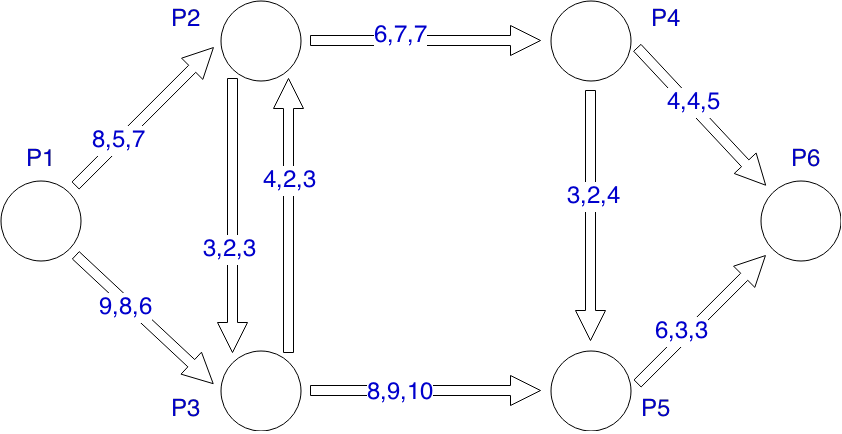
\includegraphics[width=.55\textwidth]{chapters/fig/leo1.png}
\caption{Grafo Exemplo para determinação de caminho mínimo}
Fonte: \cite{leonard}
\label{fig:leo1}
\end{figure}

As arestas possuem vários pesos que são os tempos de percursos previstos entre os pontos para os tempos
futuros $t + 1$, $t + 2$ e $t + 3$. Esses custos são armazenados no algoritmo através de um vetor de atributos.
Para determinar o caminho mínimo, utiliza-se um conjunto chamado PERM, que inicialmente contém o vértice fonte P1.
A qualquer momento PERM contém todos os vértices para os quais já foram determinados os menores caminhos usando
apenas vértices em PERM, a partir de P1. Para cada vértice $s$ fora de PERM mantém-se a menor distância dentro do
seu respectivo intervalo de previsão dist[$s$] de P1 a $s$ usando caminhos onde o único vértice que não está em
PERM seja $s$ \cite{leonard}.

Outra característica do algoritmo é a necessidade de armazenar o vértice adjacente
a $s$ neste caminho em path[$s$]. Selecionando o vértice com menor distância, entre todos os que ainda não pertencem
a PERM, adiciona ele a PERM, chamando-o de $current$, e recalcula-se as distâncias (dist) para todos os vértices
adjacentes a ele que não estejam em PERM, pois pode haver um caminho menor a partir de P1, passando por $current$, 
doo que aquele que havia antes de $current$ ser agregado a PERM. É preciso atualizar path[$s$] se houver um caminho
mais curto, e com isso indicar que $current$ é o vértice adjacente a $s$ pelo novo caminho mínimo \cite{leonard}.

Para determinar o caminho mínimo é preciso definir o ponto de origem ou nó raiz. A partir disso, o algoritmo
aplica custo de valor tendendo ao infinito a todos os vértices exceto P1, que possui custo 0. A figura \ref{fig:leo2} exibe
o ponto de saída o vértice P1.

\begin{figure}[htbp]
\centering
 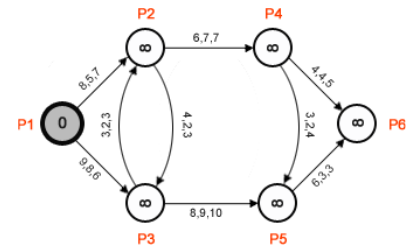
\includegraphics[width=.55\textwidth]{chapters/fig/leo2.png}
\caption{Processo de determinação de caminho mínimo - Parte 1}
Fonte: \cite{leonard}
\label{fig:leo2}
\end{figure}
\FloatBarrier
\begin{table}[htbp]
	\centering
	\begin{tabular}{l l l l}
	\toprule
	Vértice & PERM & Distância & Predecessor\\
	\midrule
	P1 & Sim & 0 & - \\
	P2 & Não & $\infty$ & - \\
	P3 & Não & $\infty$ & - \\
	P4 & Não & $\infty$ & - \\
	P5 & Não & $\infty$ & - \\
	P6 & Não & $\infty$ & - \\
	\bottomrule
	\end{tabular}
\caption{Processo de determinação de caminho mínimo - Parte 1}
 \label{tab:leotab1}
\end{table}

A partir de P1 consulta-se os vértices adjacentes a ele, que são P2 e P3. Para todos os vértices
adjacentes denonimados $s$, calcula-se o pseudocódigo da figura \ref{fig:diMod}.

\fbox{\begin{minipage}{70ex}
\vspace*{-1mm} \phantom{} \hspace{3ex} {\bf Se} dist[s] > dist[d]\ + peso(d,s)\\
\vspace*{-1mm} \phantom{} \hspace{6ex} dist[s] = dist[d]\ + peso(d,s)\\
\vspace*{-1mm} \phantom{} \hspace{6ex} path[s] = s\\
\vspace*{-1mm} \phantom{} \hspace{3ex} {\bf Fim Se}\\
\end{minipage}}
\begin{figure}[htbp]
\centering
\caption{Dijkstra Modificado - Trecho aplicado a vértices adjacentes}
\label{fig:diMod}
\end{figure}

\begin{figure}[htbp]
\centering
 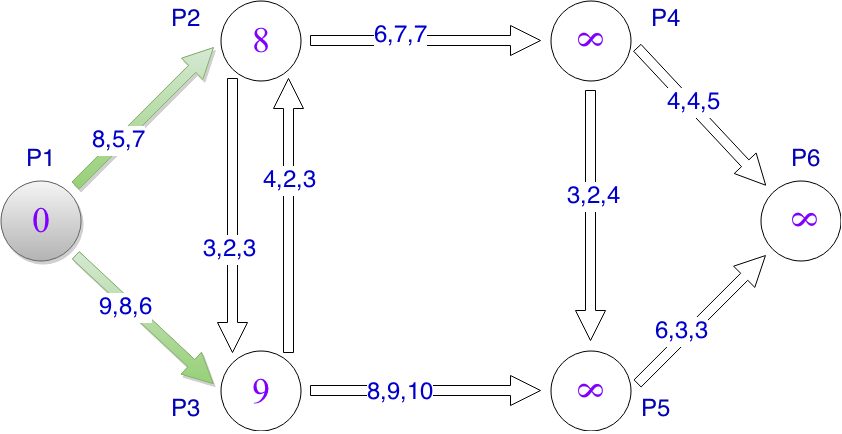
\includegraphics[width=.50\textwidth]{chapters/fig/leo3.png}
\caption{Processo de determinação de caminho mínimo - Parte 2}
Fonte: \cite{leonard}
\label{fig:leo3}
\end{figure}
\FloatBarrier
\begin{table}[htbp]
	\centering
	\begin{tabular}{l l l l}
	\toprule
	Vértice & PERM & Distância & Predecessor\\
	\midrule
	P1 & Sim & 0 & - \\
	P2 & Não & 8 & P1 \\
	P3 & Não & 9 & P1 \\
	P4 & Não & $\infty$ & - \\
	P5 & Não & $\infty$ & - \\
	P6 & Não & $\infty$ & - \\
	\bottomrule
	\end{tabular}
\caption{Processo de determinação de caminho mínimo - Parte 2}
 \label{tab:leotab2}
\end{table}

P2 é selecionado de PERM, pois possui a menor distância dist[x] = 8. Então inclui-se x em PERM e consulta-se
seus vértices adjacentes, que no caso são P3 e P4.

\begin{figure}[htbp]
\centering
 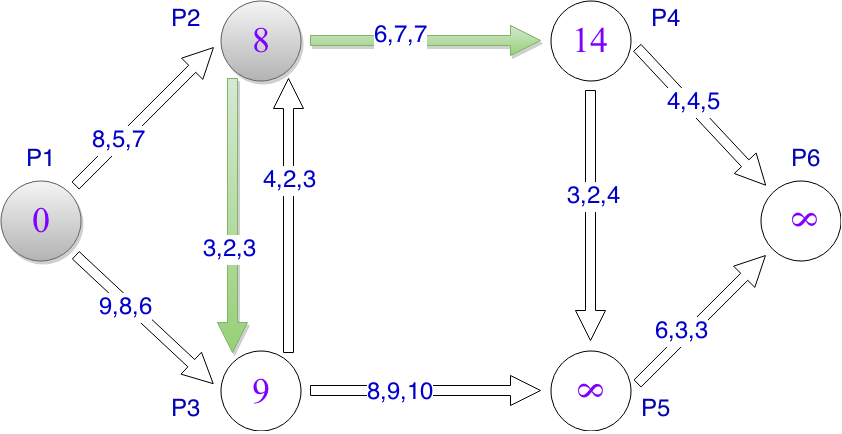
\includegraphics[width=.50\textwidth]{chapters/fig/leo4.png}
\caption{Processo de determinação de caminho mínimo - Parte 3}
Fonte: \cite{leonard}
\label{fig:leo4}
\end{figure}
\FloatBarrier
\begin{table}[htbp]
	\centering
	\begin{tabular}{l l l l}
	\toprule
	Vértice & PERM & Distância & Predecessor\\
	\midrule
	P1 & Sim & 0 & - \\
	P2 & Sim & 8 & P1 \\
	P3 & Não & 9 & P1 \\
	P4 & Não & 14 & P2 \\
	P5 & Não & $\infty$ & - \\
	P6 & Não & $\infty$ & - \\
	\bottomrule
	\end{tabular}
\caption{Processo de determinação de caminho mínimo - Parte 3}
 \label{tab:leotab3}
\end{table}

\begin{figure}[htbp]
\centering
 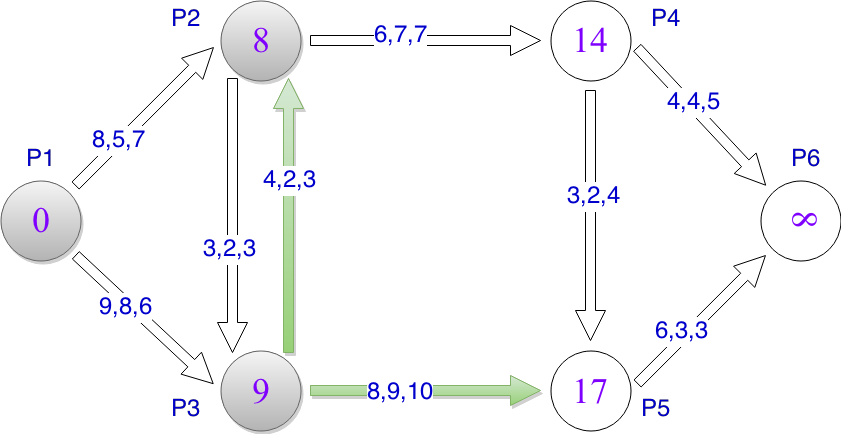
\includegraphics[width=.50\textwidth]{chapters/fig/leo5.png}
\caption{Processo de determinação de caminho mínimo - Parte 4}
Fonte: \cite{leonard}
\label{fig:leo5}
\end{figure}
\FloatBarrier
\begin{table}[htbp]
	\centering
	\begin{tabular}{l l l l}
	\toprule
	Vértice & PERM & Distância & Predecessor\\
	\midrule
	P1 & Sim & 0 & - \\
	P2 & Sim & 8 & P1 \\
	P3 & Sim & 9 & P1 \\
	P4 & Não & 14 & P2 \\
	P5 & Não & 17 & P3 \\
	P6 & Não & $\infty$ & - \\
	\bottomrule
	\end{tabular}
\caption{Processo de determinação de caminho mínimo - Parte 4}
 \label{tab:leotab4}
\end{table}

Ao selecionar o vértice P4, não pertencente a PERM, o intervalo de previsão é ultrapassado
de 10 minutos. Logo, é utilizada a segunda posição do vetor de custos $t + 2$. O custo do trajeto até
o vértice P5 pelo P4 é menor do que o custo atual por P3, logo atualiza-se seu peso e predecessor
para 16 e P4 respectivamente.

\begin{figure}[htbp]
\centering
 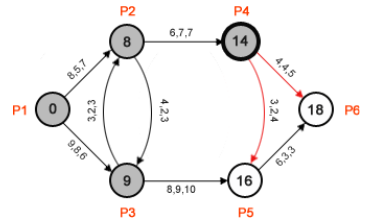
\includegraphics[width=.50\textwidth]{chapters/fig/leo6.png}
\caption{Processo de determinação de caminho mínimo - Parte 5}
Fonte: \cite{leonard}
\label{fig:leo6}
\end{figure}
\FloatBarrier
\begin{table}[htbp]
	\centering
	\begin{tabular}{l l l l}
	\toprule
	Vértice & PERM & Distância & Predecessor\\
	\midrule
	P1 & Sim & 0 & - \\
	P2 & Sim & 8 & P1 \\
	P3 & Sim & 9 & P1 \\
	P4 & Sim & 14 & P2 \\
	P5 & Não & 16 & P4 \\
	P6 & Não & 18 & P4 \\
	\bottomrule
	\end{tabular}
\caption{Processo de determinação de caminho mínimo - Parte 5}
 \label{tab:leotab5}
\end{table}

P5 é adicionado a PERM e seu único vértice adjacente é P6. Logo temos:

\begin{figure}[htbp]
\centering
 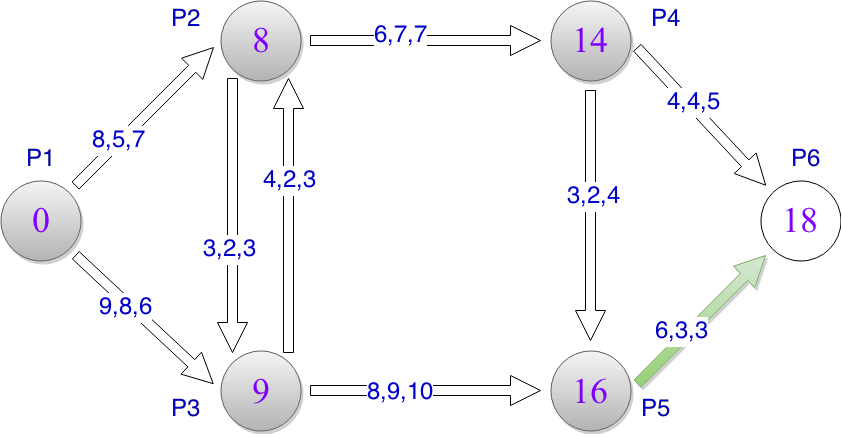
\includegraphics[width=.50\textwidth]{chapters/fig/leo7.png}
\caption{Processo de determinação de caminho mínimo - Parte 6}
Fonte: \cite{leonard}
\label{fig:leo7}
\end{figure}
\FloatBarrier
\begin{table}[htbp]
	\centering
	\begin{tabular}{l l l l}
	\toprule
	Vértice & PERM & Distância & Predecessor\\
	\midrule
	P1 & Sim & 0 & - \\
	P2 & Sim & 8 & P1 \\
	P3 & Sim & 9 & P1 \\
	P4 & Sim & 14 & P2 \\
	P5 & Sim & 16 & P4 \\
	P6 & Sim & 18 & P4 \\
	\bottomrule
	\end{tabular}
\caption{Processo de determinação de caminho mínimo - Parte 6}
 \label{tab:leotab5}
\end{table}

E finalmente temos a figura \ref{fig:leo8}, pois P6 não possui vértice adjacente. Logo, o 
tempo para percorrer o caminho mínimo passando por P1, P2, P4 e P6 é 18 minutos.

\begin{figure}[htbp]
\centering
 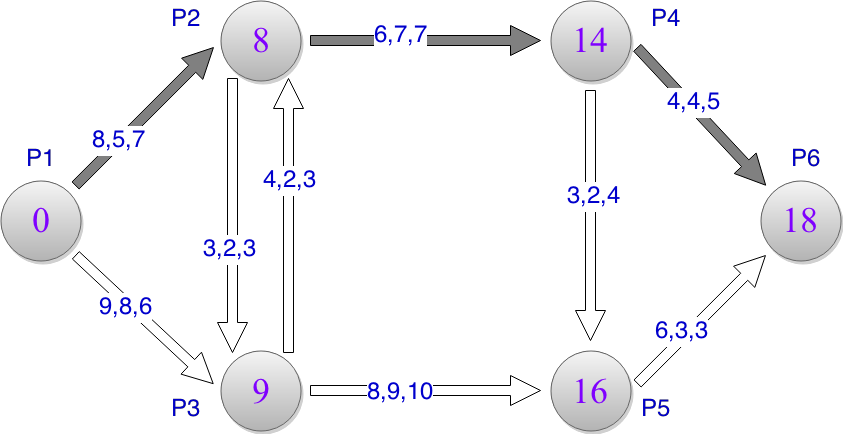
\includegraphics[width=.50\textwidth]{chapters/fig/leo8.png}
\caption{Processo de determinação de caminho mínimo - Parte 7}
Fonte: \cite{leonard}
\label{fig:leo8}
\end{figure}
\FloatBarrier

% Atributos dinamicos e topologia estáticos com limite inferior - monografia
\subsubsection{Topologia Dinâmica e Atributos Estáticos}

\subsubsection{Topologia Dinâmica e Atributos Dinâmicos}
% Atributos dinamicos e topologia dinâmica com limite inferior - monografia




























\chapter{Validação}

Para validação dos algoritmos foram gerados alguns grafos hipotéticos com cenários distintos.
Alguns deles utilizaram o mesmo vetor de custo, como dito na seção \ref{sec:pathdyn}, que representam
o tempo médio das passagens dos veículos por uma aresta ao longo do dia, em intervalos de 10 minutos.

% \subsection{Cenários de teste}

\section{Ferramenta de simulação do caminho mínimo}
Para determinar o caminho mínimo entre dois pontos conhecidos em grafos dinâmicos, foi criado
uma extensão ao Dynagraph, que simula o caminho mínimo. Para isso, segue a sequência:
\begin{itemize}
\item Ler a estrutura de dados JSON;
\item Exibir o grafo com todos os vértices e arestas;
\item Selecionar um dos 3 algoritmos para cálculo e exibição do caminho mínimo;
\item Baixar o arquivo JSON ou ir para a aplicação Dynagraph, que contém os mesmos dados do grafo mais as arestas do caminho mínimo;
\end{itemize}

As figuras \ref{fig:shortestpath}, \ref{fig:upperlimit} e \ref{fig:downlimit} mostram captura de telas
da ferramenta exibindo exemplos de caminho mínimo dos 3 algoritmos e os seus dados:

\begin{figure}[htbp]
\centering
 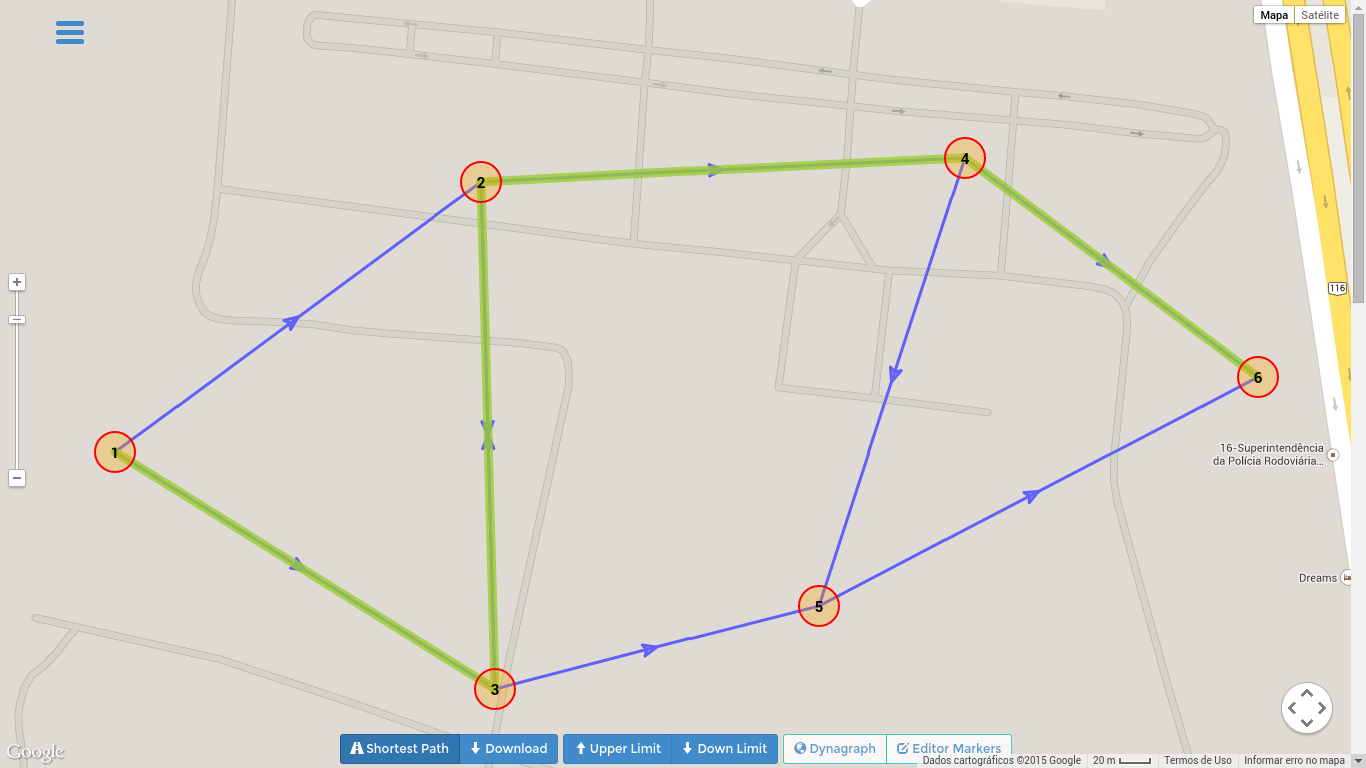
\includegraphics[width=.90\textwidth]{chapters/fig/validacao/shortestpath.png}
\caption{Simulador de Caminho Mínimo - Topologia Dinâmica e Atributos Dinâmicos}
\label{fig:shortestpath}
\end{figure}
\FloatBarrier

\begin{figure}[htbp]
\centering
 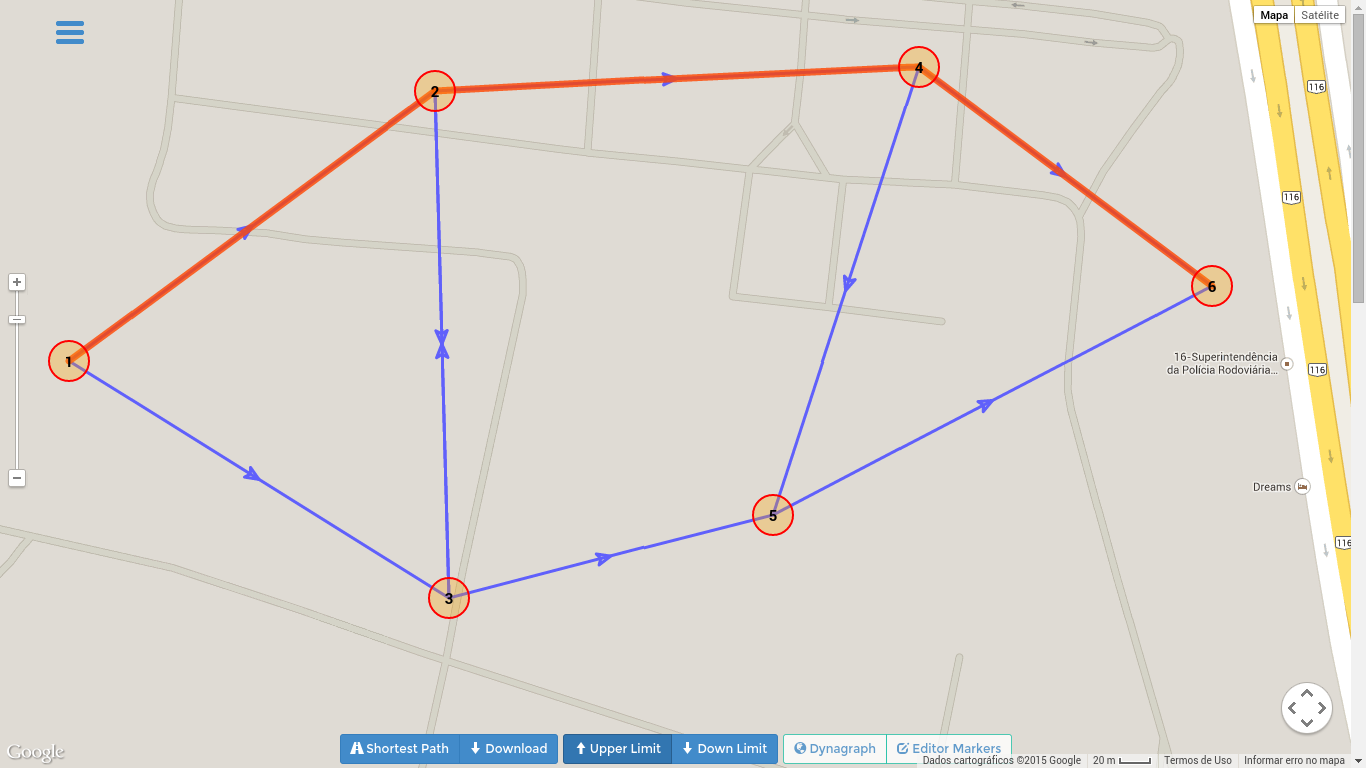
\includegraphics[width=.90\textwidth]{chapters/fig/validacao/upperlimit.png}
\caption{Simulador de Caminho Mínimo - Topologia Estática e Atributos Dinâmicos}
\label{fig:upperlimit}
\end{figure}
\FloatBarrier

\begin{figure}[htbp]
\centering
 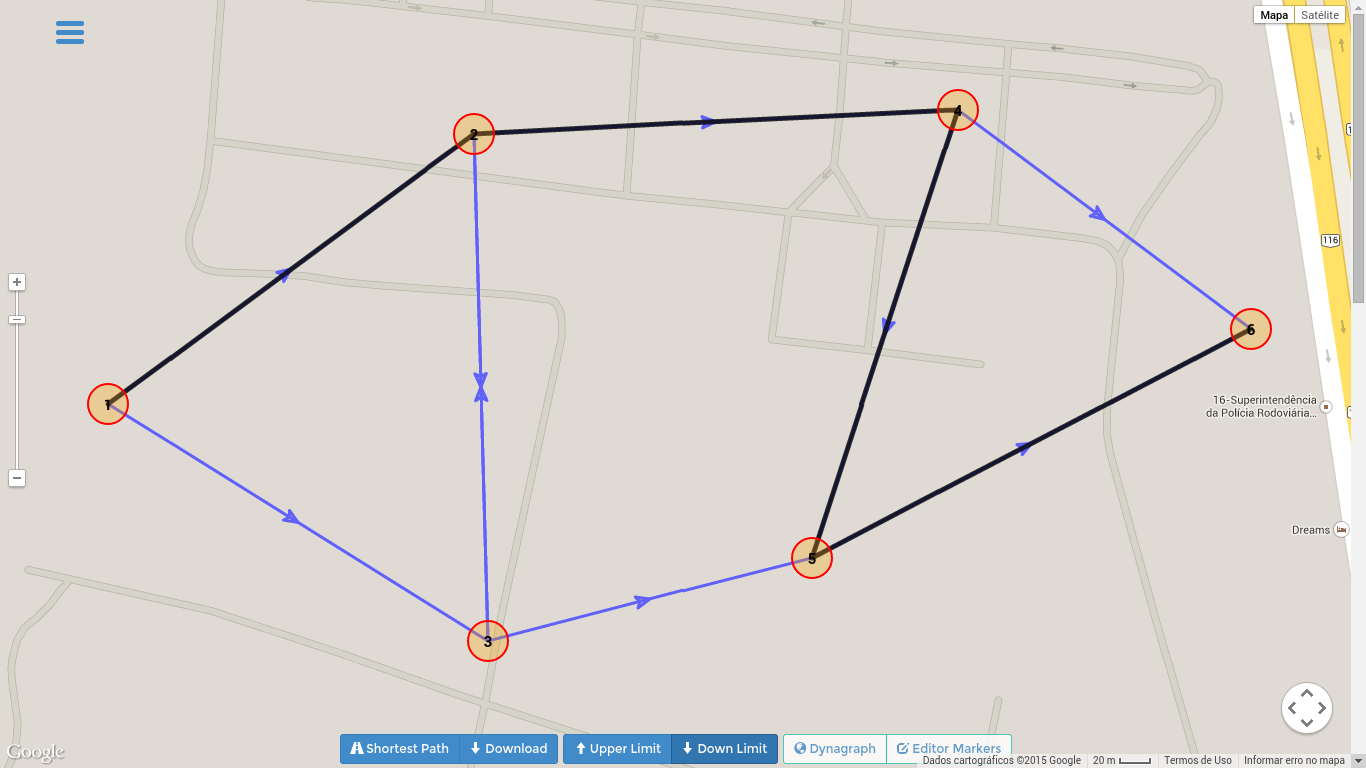
\includegraphics[width=.90\textwidth]{chapters/fig/validacao/downlimit.png}
\caption{Simulador de Caminho Mínimo - Topologia Estática e Atributos Dinâmicos: mesma abordagem em \cite{leonard}}
\label{fig:downlimit}
\end{figure}
\FloatBarrier

\begin{center}
  \line(1,0){450}
\end{center}
\lstinputlisting[language=Java]{chapters/dataex1.json}
\begin{figure}[htbp]
  \begin{center}
    \line(1,0){450}
  \end{center}
  \centering
  \caption{Estrutura JSON - Exemplo 1}
  \label{fig:jsondyn}
\end{figure}
\FloatBarrier

A seguir, são apresentados os grafos gerados pela ferramenta de simulação com seus respectivos dados,
e a exibição do caminho mínimo no Dynagraph. As figuras seguem a ordem da esquerda para a direita e
de cima para baixo.

\begin{figure}[htbp]
\centering
 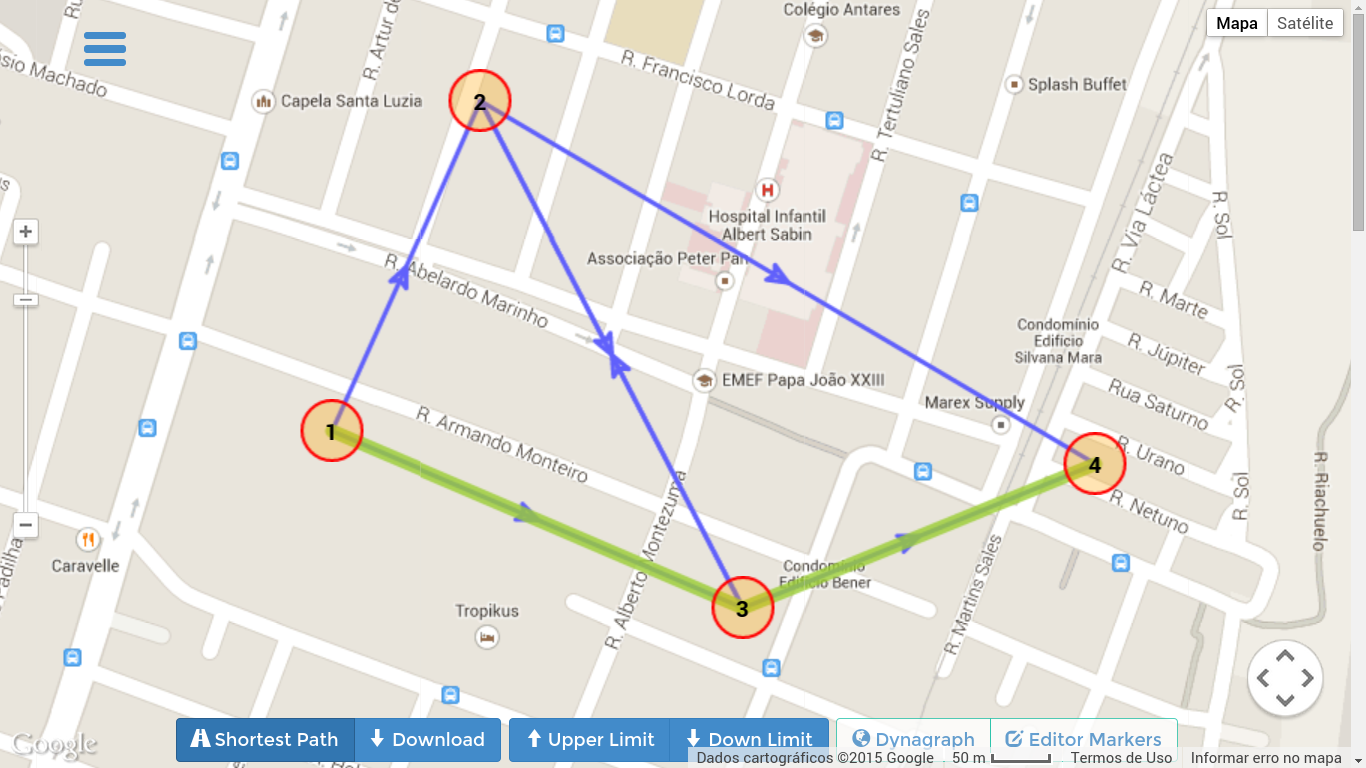
\includegraphics[width=.70\textwidth]{chapters/fig/validacao/ex1.png}
\caption{Simulador de Caminho Mínimo - Exemplo 1}
\label{fig:ex1}
\end{figure}
\FloatBarrier

\begin{figure}[htbp]
\centering
 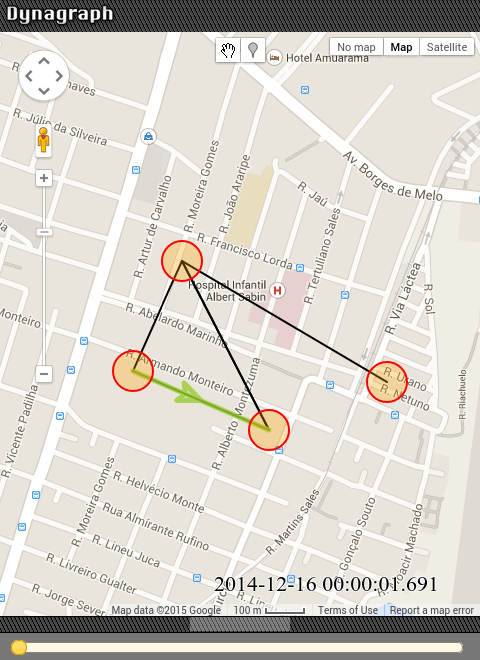
\includegraphics[width=.35\textwidth]{chapters/fig/validacao/dyn1a.png}
 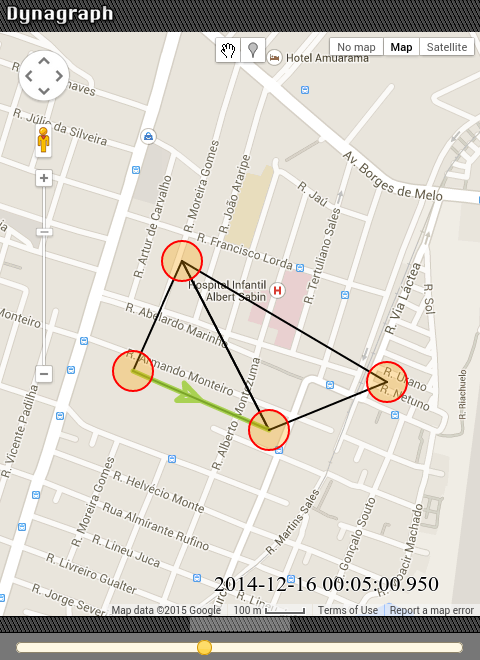
\includegraphics[width=.35\textwidth]{chapters/fig/validacao/dyn1b.png}
 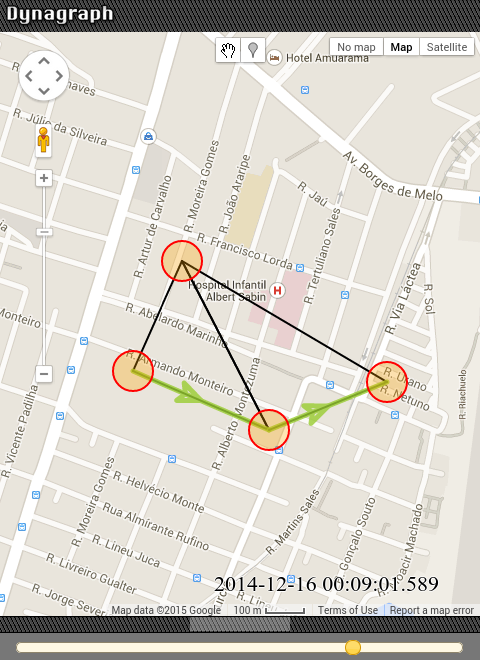
\includegraphics[width=.35\textwidth]{chapters/fig/validacao/dyn1c.png}
 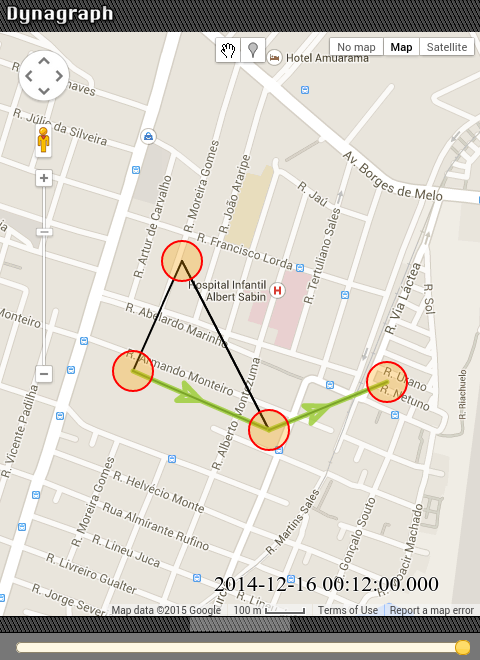
\includegraphics[width=.35\textwidth]{chapters/fig/validacao/dyn1d.png}
\caption{Caminho Mínimo no Dynagraph - Exemplo 1}
\label{fig:dyn1}
\end{figure}
\FloatBarrier

\begin{center}
  \line(1,0){450}
\end{center}
\lstinputlisting[language=Java]{chapters/fig/validacao/dyn1.json}
\begin{figure}[htbp]
  \begin{center}
    \line(1,0){450}
  \end{center}
  \centering
  \caption{Simulador de Caminho Mínimo: Estrutura JSON - Exemplo 1}
  \label{fig:jsondyn1}
\end{figure}
\FloatBarrier


\begin{figure}[htbp]
\centering
 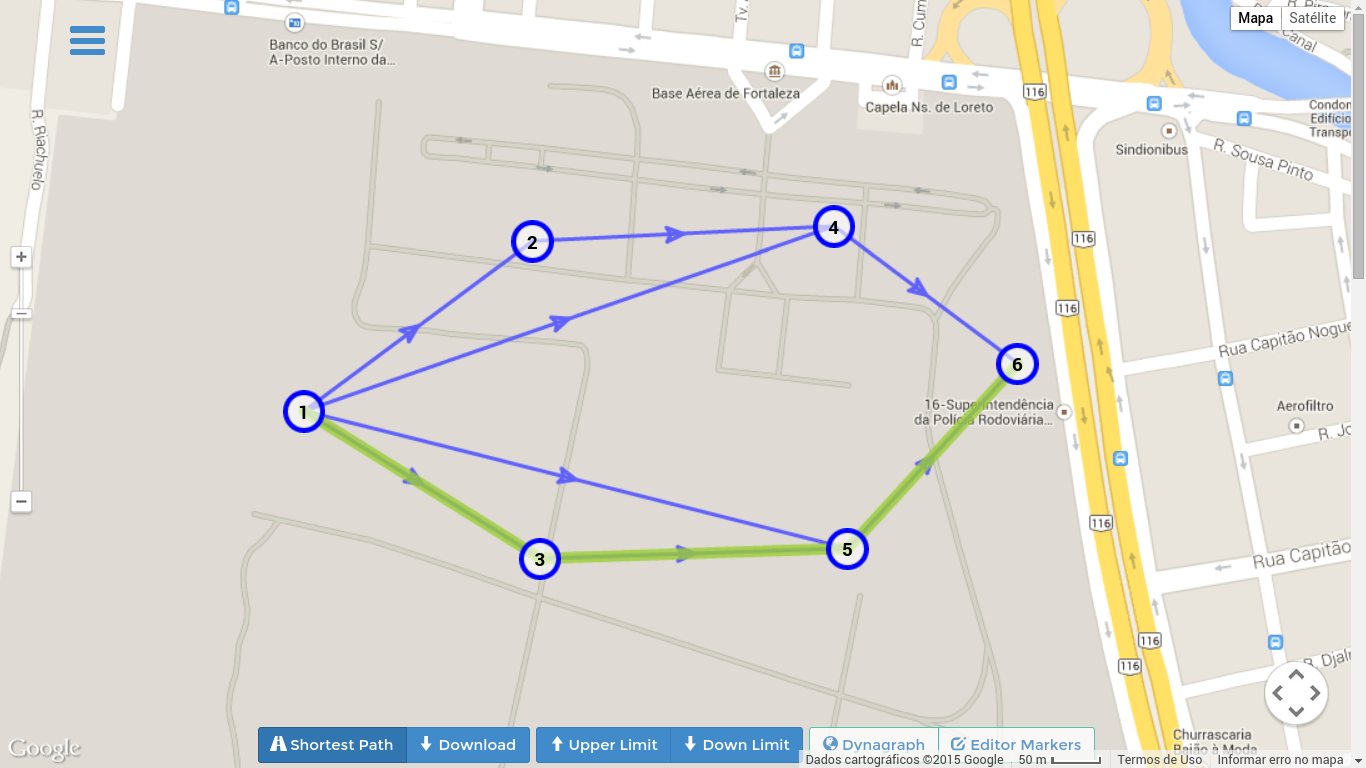
\includegraphics[width=.70\textwidth]{chapters/fig/validacao/ex2.png}
\caption{Simulador de Caminho Mínimo - Exemplo 2}
\label{fig:ex2}
\end{figure}
\FloatBarrier

\begin{figure}[htbp]
\centering
 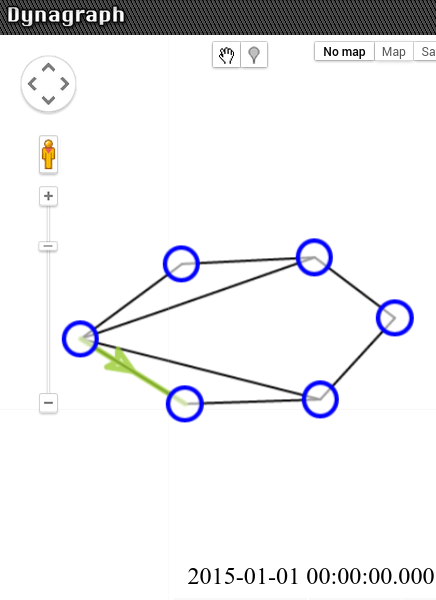
\includegraphics[width=.35\textwidth]{chapters/fig/validacao/dyn2a.png}
 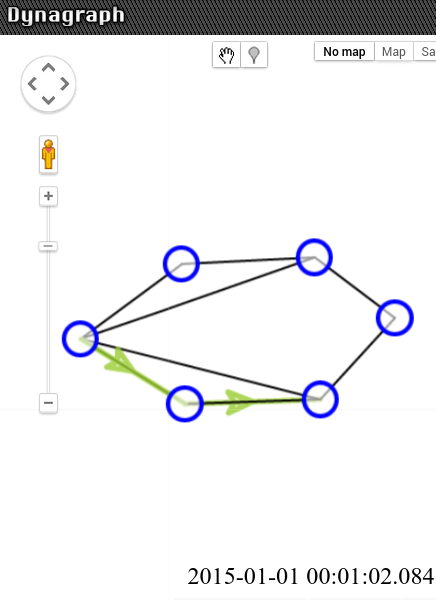
\includegraphics[width=.35\textwidth]{chapters/fig/validacao/dyn2b.png}
 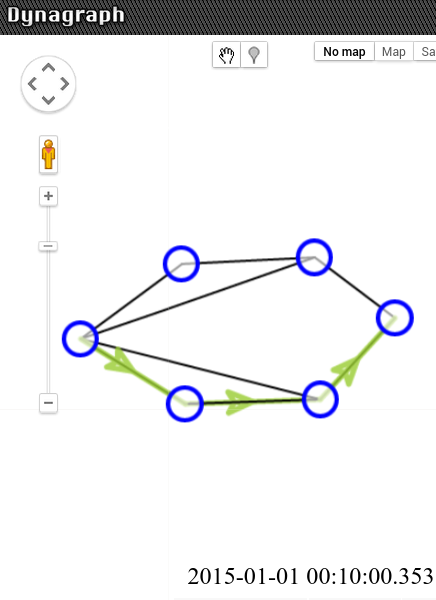
\includegraphics[width=.35\textwidth]{chapters/fig/validacao/dyn2c.png}
 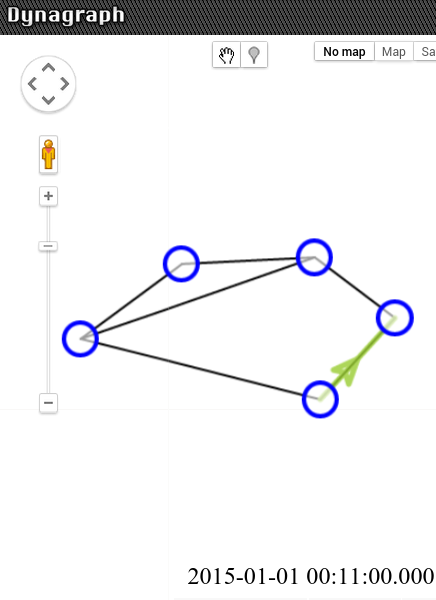
\includegraphics[width=.35\textwidth]{chapters/fig/validacao/dyn2d.png}
\caption{Caminho Mínimo no Dynagraph - Exemplo 2}
\label{fig:dyn2}
\end{figure}
\FloatBarrier

\begin{center}
  \line(1,0){450}
\end{center}
\lstinputlisting[language=Java]{chapters/fig/validacao/dyn2.json}
\begin{figure}[htbp]
  \begin{center}
    \line(1,0){450}
  \end{center}
  \centering
  \caption{Simulador de Caminho Mínimo: Estrutura JSON - Exemplo 2}
  \label{fig:jsondyn2}
\end{figure}
\FloatBarrier

A seguir, o mesmo exemplo do grafo anterior, mas com o horário de início do percurso diferente.
Percebe-se que a hora é ultrapassada, pois o percurso inicia às 23 horas e 50 minutos.
% Considerando o grafo G(N=\{P1, P2, P3, P4, P5, P6\}, A), o caminho determinado parte de P1, passa por P4 e chega em P6.

\begin{figure}[htbp]
\centering
 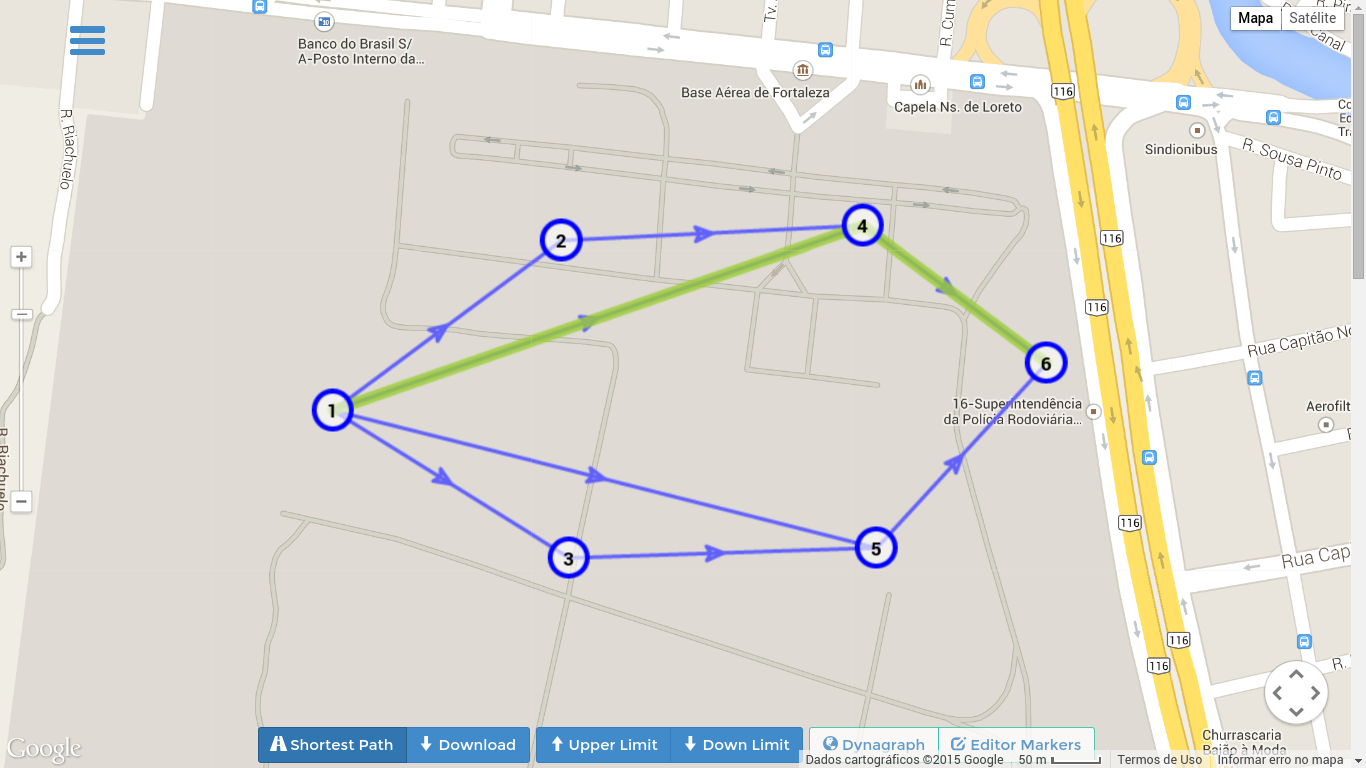
\includegraphics[width=.70\textwidth]{chapters/fig/validacao/ex3.png}
\caption{Simulador de Caminho Mínimo - Exemplo 3}
\label{fig:ex3}
\end{figure}
\FloatBarrier

\begin{figure}[htbp]
\centering
 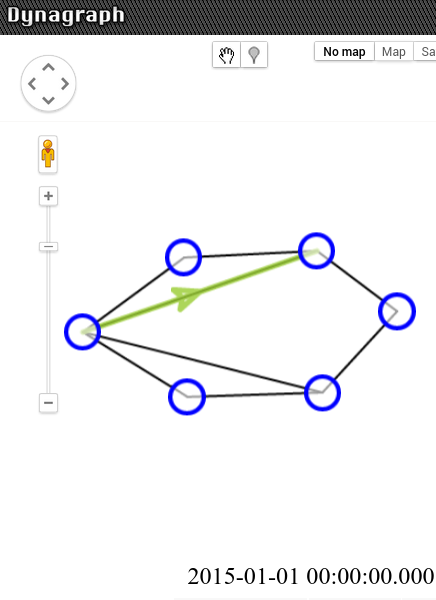
\includegraphics[width=.35\textwidth]{chapters/fig/validacao/dyn3a.png}
 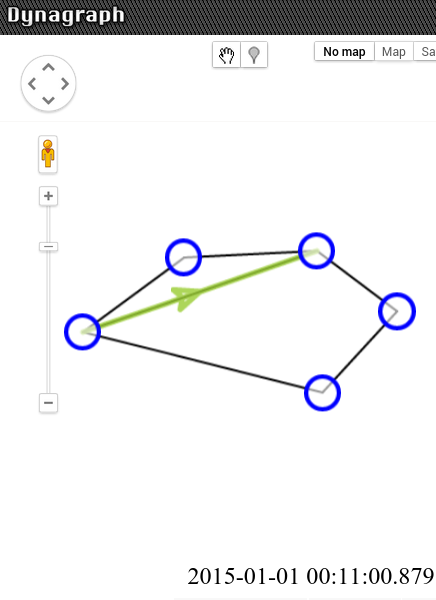
\includegraphics[width=.35\textwidth]{chapters/fig/validacao/dyn3b.png}
 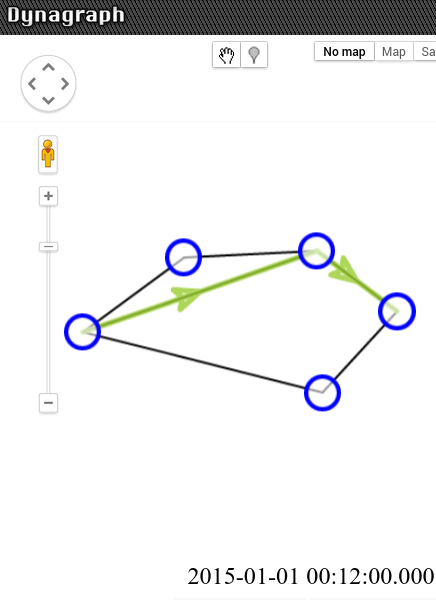
\includegraphics[width=.35\textwidth]{chapters/fig/validacao/dyn3c.png}
\caption{Caminho Mínimo no Dynagraph - Exemplo 3}
\label{fig:dyn3}
\end{figure}
\FloatBarrier

\begin{center}
  \line(1,0){450}
\end{center}
\lstinputlisting[language=Java]{chapters/fig/validacao/dyn3.json}
\begin{figure}[htbp]
  \begin{center}
    \line(1,0){450}
  \end{center}
  \centering
  \caption{Simulador de Caminho Mínimo: Estrutura JSON - Exemplo 3}
  \label{fig:jsondyn3}
\end{figure}
\FloatBarrier

Logo abaixo, um exemplo usando o mesmo vetor de custo do exemplo 3.

\begin{figure}[htbp]
\centering
 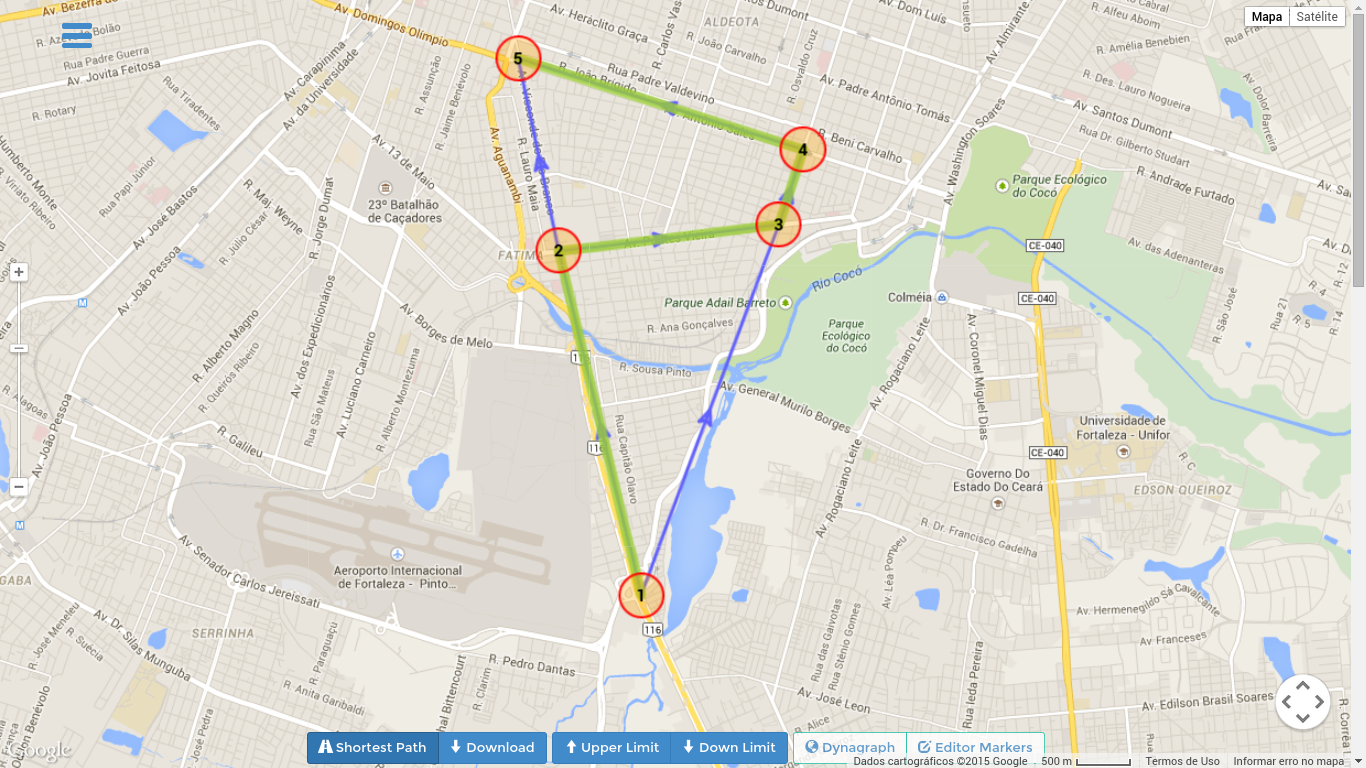
\includegraphics[width=.70\textwidth]{chapters/fig/validacao/ex4.png}
\caption{Simulador de Caminho Mínimo - Exemplo 4}
\label{fig:ex4}
\end{figure}
\FloatBarrier

\begin{figure}[htbp]
\centering
 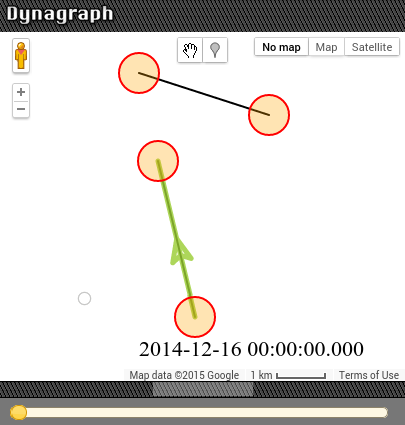
\includegraphics[width=.35\textwidth]{chapters/fig/validacao/dyn4a.png}
 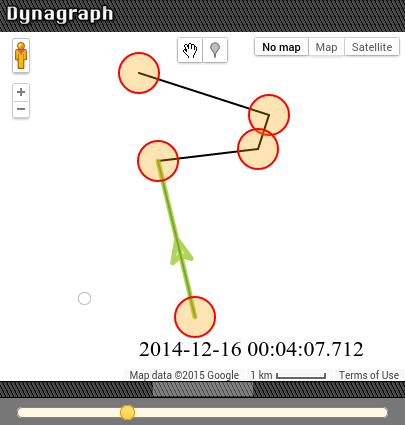
\includegraphics[width=.35\textwidth]{chapters/fig/validacao/dyn4b.png}
 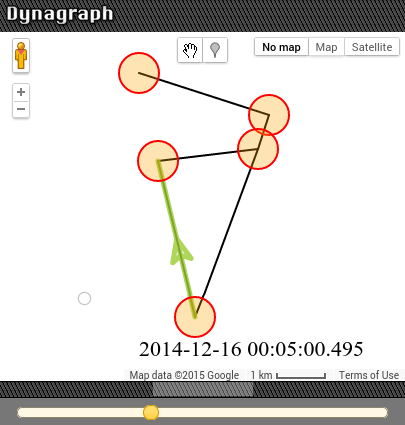
\includegraphics[width=.35\textwidth]{chapters/fig/validacao/dyn4c.png}
 \includegraphics[width=.35\textwidth]{chapters/fig/validacao/dyn4d.png}
 \includegraphics[width=.35\textwidth]{chapters/fig/validacao/dyn4e.png}
 \includegraphics[width=.35\textwidth]{chapters/fig/validacao/dyn4f.png}
 \includegraphics[width=.35\textwidth]{chapters/fig/validacao/dyn4g.png}
 \includegraphics[width=.35\textwidth]{chapters/fig/validacao/dyn4h.png}
\caption{Caminho Mínimo no Dynagraph - Exemplo 4}
\label{fig:dyn4}
\end{figure}
\FloatBarrier

\begin{center}
  \line(1,0){450}
\end{center}
\lstinputlisting[language=Java]{chapters/fig/validacao/dyn4.json}
\begin{figure}[htbp]
  \begin{center}
    \line(1,0){450}
  \end{center}
  \centering
  \caption{Simulador de Caminho Mínimo: Estrutura JSON - Exemplo 4}
  \label{fig:jsondyn4}
\end{figure}
\FloatBarrier

\chapter{Conclusão e Trabalhos Futuros}

O presente trabalho utilizou algoritmos de caminho mínimo em grafos dinâmicos
para determinação de percusos com tempo mínimo em grafos hipotéticos.
A aplicação destes algoritmos resultou na formulação de um modelo computacional em grafos
de topologia dinâmica e atributos dinâmicos. Também foi construída uma ferramenta (\textit{software})
extendida do Dynagraph, que calcula e exibe o caminho mínimo entre dois vértices conhecidos.

Inicialmente foram apresentados os algoritmos de topologia estática e atributos dinâmicos com
limite inferior e superior. Em seguida, esses mesmos algoritmos foram utilizados no algoritmo
de topologia dinâmica e atributos dinâmicos.

Pode-se concluir que o algoritmo utilizado em grafos de topologia dinâmica e atributos dinâmicos
é eficiente ao ponto de garantir a resolução do problema dentro dos objetivos propostos, pois ele
garante um intervalo de previsão para travessia de cada aresta e intervalo para o caminho mínimo.
Mesmo sabendo que o modelo não é o mais eficiente, pois o mesmo é implementado usando o
algoritmo de Dijkstra com Radix Heap, e poderia usar a estrutura de dados Fibonacci heap com a
implementação do radix heap, e com isso reduzir ainda mais a complexidade.

Esta pesquisa também contribuiu com a integração da ferramenta implementada com a ferramenta Dynagraph.
Essa integração permite através do Dynagraph solicitar o caminho mínimo do grafo em análise. Para isso, ele faz 
uma chamada ao \textit{software} deselvolvido. Este, por sua vez, analisa o grafo enviado, calcula o caminho mínimo
e envia para o Dynagraph o mesmo grafo acrescido das arestas do caminho mínimo gerado.

Para trabalho futuros, pretende-se provar que o algoritmo de caminho mínimo para grafos dinâmicos implementado garante que o
intervalo de previsão é mínimo. Também pretende-se otimizar o algoritmo para garantir o cálculo eficiente, pois a pesquisa
somente se concentrou na elaboração do modelo computacional.
Para trabalhos futuros na ferramenta, pretende-se resolver alguns detalhes para garantir o funcionamento da ferramenta.
A aplicação ainda limita-se ao selecionar um grafo em arquivo externo, pois o mesmo seleciona um grafo na implementação.
Pretende-se disponibilizar uma opção na ferramenta que indique o horário inicial de partida
do caminho mínimo. E por fim, aperfeiçoar o Editor de Características extendendo a edição para arestas e integrar ao Dynagraph.


% bibliografia
\bibliography{references}

\end{document}

